
% Autor: Tomáš Majerech
\chapter{Úvod}
Každé čtyři roky stojí obyvatelé České republiky před rozhodnutím, komu dají svůj hlas ve volbách do Poslanecké sněmovny. Velké množství z nich nemá mnohdy čas ani chuť pravidelně sledovat dění na politické scéně a nejsou si tudíž jistí, kdo z kandidátů či stran by dostatečně dobře zastupoval jejich názory a zájmy. Proto stále častěji lidé vyhledávají volební kalkulačky, kde můžou pomocí odpovědí na pár otázek zjistit shodu s některým z kandidátů nebo s některou ze stran. Na tomto již existujícím principu staví také tato bakalářská práce a dále ho rozšiřuje a modernizuje. 
\par Skutečnost, že lidé volební kalkulačky pravidelně využívají, skýtá prostor k potenciálnímu budoucímu využítí této práce širokou veřejností a její existence by tedy nekončila ve školním archivu, nýbrž by se mohla stát univerzálním nástrojem, usnadňujícím život řadě běžných lidí. To byl také jeden z důvodů, proč mi toto téma dávalo smysl.
\par Ve druhé kapitole (\ref{chap:Prerekvizity}) je čtenář seznámen s problematikou legislativního procesu v České republice, strukturou Poslanecké sněmovny a základními pojmy nutnými k porozumění této práci. Také je zde popsána existující konkurence (v době psaní této práce) a zdroj dat. Třetí kapitola (\ref{chap:technologie}) rozebírá použité technologie. Kromě HTML a CSS, které se nachází prakticky na každém webu, jsem se rozhodl pro tuto práci využít na frontendu framework Bootstrap a css preprocessor SASS. Na backendové části je využit python framework Django. K uložení dat je využita objektově-relační databáze PostgreSQL. Ve čtvrté kapitole (\ref{chap:navrh}) je popsán postup návrhu webového rozhraní a struktury uložených dat.\\

\todo{popis toho co v bp je}









\chapter{Prerekvizity}
\label{chap:Prerekvizity}
V úvodu této kapitoly jsou stručně shrnuty základní pojmy a procesy týkající se zaměření této práce, zejména z oblasti legislativního procesu. V další části jsou zmíněny již existující konkurenční řešení a jejich nedostatky. Následuje popis primárního zdroje dat.


\section{Základní pojmy}

\subsection{Poslanecká sněmovna}
Poslanecká sněmovna je jedna ze dvou složek, tzv. komor, Parlamentu České republiky. Má 200 členů, tzv. poslanců, volených v přímé volbě na 4 roky. \cite{ustava-parlament} \\
Smyslem Poslanecké sněmovny je tvorba a přijímání zákonů. Ty můžou přijít od poslanců, jejich skupin, krajských zastupitelstev, senátu a vlády. \cite{ustava-navrh_zakona} \\
Schvalování zákonů má 3 části zvané čtení.
\begin{enumerate}
    \item čtení: \\
    Rozhoduje se o tom, jestli se PS bude návrhem vůbec zabývat. Pokud projde, dochází k dalšímu hlasování o tom, jakému výboru bude návrh přiřazen k přezkoumání.
    V některých případech může být návrh schválen PS už v této fázi, pokud o to navrhovatel požádá.
    \item čtení: \\
    Na začátku vystoupí jeden zpravodaj z každého přiřazeného výboru a informuje PS zprávou a doporučením, na kterém se výbor usnesl. Také se přednáší pozměňovací návrhy.
    \item čtení: \\
    Hlasuje se o pozměňovacích návrzích ze 2. čtení, případně o jiných návrzích. Následuje hlasování o přijetí zákona jako celku.\\
    Po přijetí pokračuje návrh do senátu, což je druhá komora Parlamentu České republiky. Ten může návrh odmítnout a vrátit zpět do PS. V takovém případě musí PS o návrhu opět hlasovat a pokud je návrh schválen nadpoloviční většinou všech poslanců (101 hlasů), je senát přehlasován. Posledním krokem je podpis prezidenta České republiky. Ten má ale opět právo návrh vetovat. Zde je postup stejný jako u veta senátního a PS ho může opět přehlasovat nadpoloviční většinou všech poslanců.
\end{enumerate}
Zjednodušený průběh legislativního procesu je znázorněn na obrázku \ref{fig:legislativni_proces}.

\begin{figure}
    \centering
    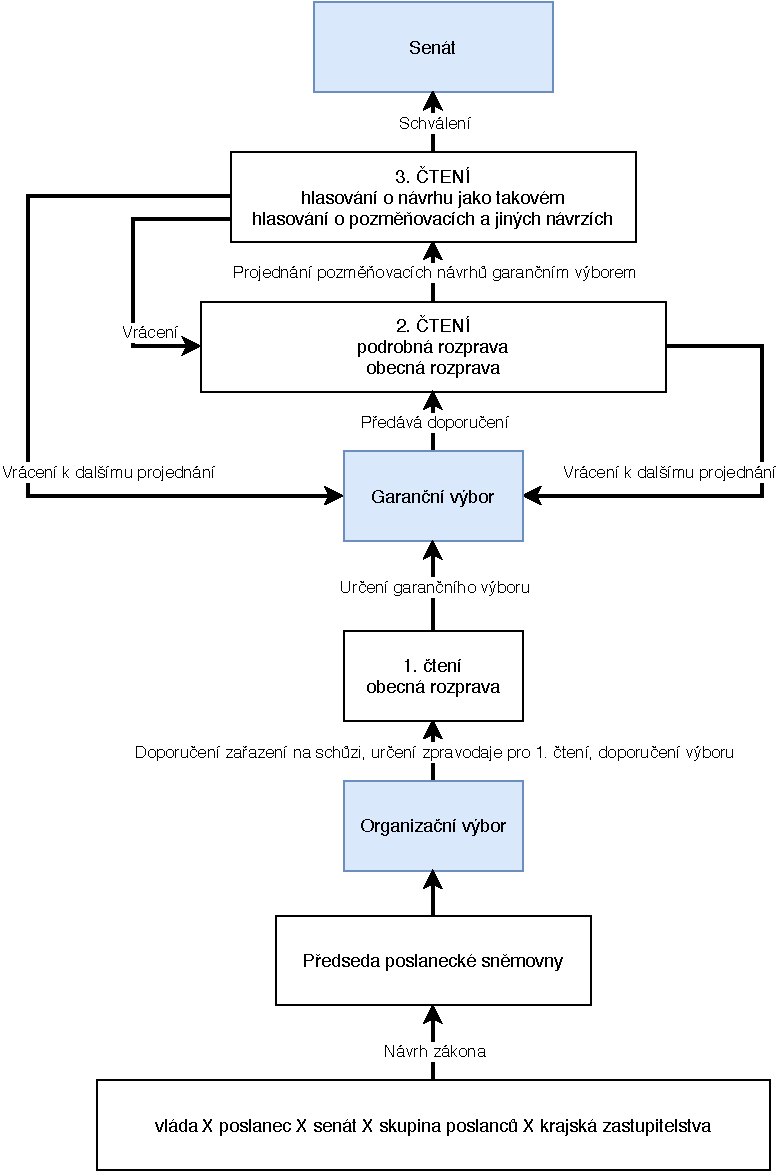
\includegraphics[width=0.9\textwidth]{obrazky-figures/legislativni_proces_my.pdf}
    \caption{Zjednodušený graf legislativního procesu v Poslanecké sněmovně}
    \label{fig:legislativni_proces}
\end{figure}
 
\subsection{Výbory poslanecké sněmovny}
\label{vybory}
\par Výbory poslanecké sněmovny jsou skupiny lidí zaměřené na určitý odborný problém, složené jak z členů vlády, tak opozice. Tyto skupiny se návrhem zákona zabývají v odborné rovině a následně na 2. čtení PS doporučí návrh přijmout, zamítnout, nebo navrhnou změny.\\
Jeden návrh může být přiřazen více výborům, každý z výborů má svého zpravodaje, ale jen jeden z nich je tzv. garanční - ručí za přidělený návrh. \\

\subsection{Jednání PS}
\par Jednání, na kterých jsou návrhy zákonů projednávány, se nazývají schůze Poslanecké sněmovny. Aby byla sněmovna usnášeníschopná, musí být přítomno alespoň třetinové kvórum, což odpovídá 67 poslancům. \cite{ustava-kvorum} \\
Průběh jednání z hlediska hlasování vypadá následovně:\\
\begin{itemize}
    \item Přihlášení účastníků
    \item Určení zapisovatelů a hlasování o jejich schválení
    \item Hlasování o jednotlivých bodech aktuální schůze \\
    - v případě, že vůbec dojde k jejich projednání
    \item Hlasování o pořadí projednávaných bodů
    \item Hlasování o konkrétních bodech na pořadu\\
    - může dojít ke zpochybnění hlasování a k jeho opakování \\
    \item V průběhu schůze může dojít také k některým dalším, méně zajímavým, hlasovnáním například o odložení projednávání nějakého aktuálního bodu na později, či vyhlášení přestávky.
    
\end{itemize}

\subsection{Kvórum}
Kvórum je minimální počet hlasů nutný pro přijetí návrhu hlasováním. Běžně je kvórum nadpoloviční většina přítomných poslanců, v některých případech se však může lišit. Například kvórum nadpoloviční většiny všech poslanců nutné pro přehlasování veta Senátu, či prezidenta, nebo kvórum 3/5 přítomných nutné pro přijetí ústavních zákonů \cite{zakon-kvorum}.

\subsection{Sněmovní tisky}
Sněmovní tisky jsou, zjednodušeně řečeno, dokumenty předkládané poslancům jako podklady pro jednotlivé body programu. 

\section{Existující řešení}
Na internetu lze v době psaní této práce nalézt více verzí českých i zahraničních volebních kalkulaček. Jelikož jsou volby obecně silně specifické v jednotlivých zemích, zahraniční aplikace zde nebudu rozebírat. Z těch českých jsou nejzajímavější hlavně volebnikalkulacka.cz\footnote{volebnikalkulacka.cz: \url{https://volebnikalkulacka.cz/}} a ta na zpravodajském portálu iDnes.cz\footnote{Volební kalkulačka na idnes.cz: \url{https://volby.idnes.cz/volebni-kalkulacka-kraje.aspx}}. Za zmínku stojí také Postvolítko\footnote{Postvolítko: \url{https://www.fi.muni.cz/~xzahrad4/Hlasovatko/index.cgi?o=8}}, projekt studentů Masarykovy univerzity. 

\subsection{volebnikalkulacka.cz}
Princip této volební kalkulačky  je jednoduchý. Autor, či autoři, vytvoří soubor otázek, který by podle jejich názoru mohl uživatele zajímat. Tyto otázky jsou následně rozeslány všem zúčastněným politickým stranám, či kandidátům. Na základě matematických modelů jsou poté odpovědi zpracovány a vybrány nejlepší otázky. Tyto jsou nakonec prezentovány v samotné kalkulačce (obr. \ref{fig:volebnikalkulacka-otazka}), kde na ně odpovídá uživatel. Po ukončení dotazníku je uživateli představena jeho procentuální shoda v odpovědích s jednotlivými stranami či kandidáty (obr. \ref{fig:volebnikalkulacka-vysledky}) \cite{volebnikalkulacka-info}.
\par Výhoda tohoto systému je v jeho jednoduchosti a přehlednosti. Otázky bývají jednoznačné, srozumitelné a týkají se aktuálních témat, takže běžný uživatel nemusí mít nic než obecný přehled o hlavním dění v České republice a ve svém kraji. 
\par Za jeho nevýhodu by se dala považovat závislost na pravdivých odpovědích a nepopulistickém přístupu. Může se totiž stát, že kandidát vyplní dotazník podle toho co zrovna v tu chvíli jeho potenciální voliči požadují a následně ve skutečných hlasováních v Poslanecké sněmovně hlasovat jinak.
\\

\begin{figure}
    \centering
    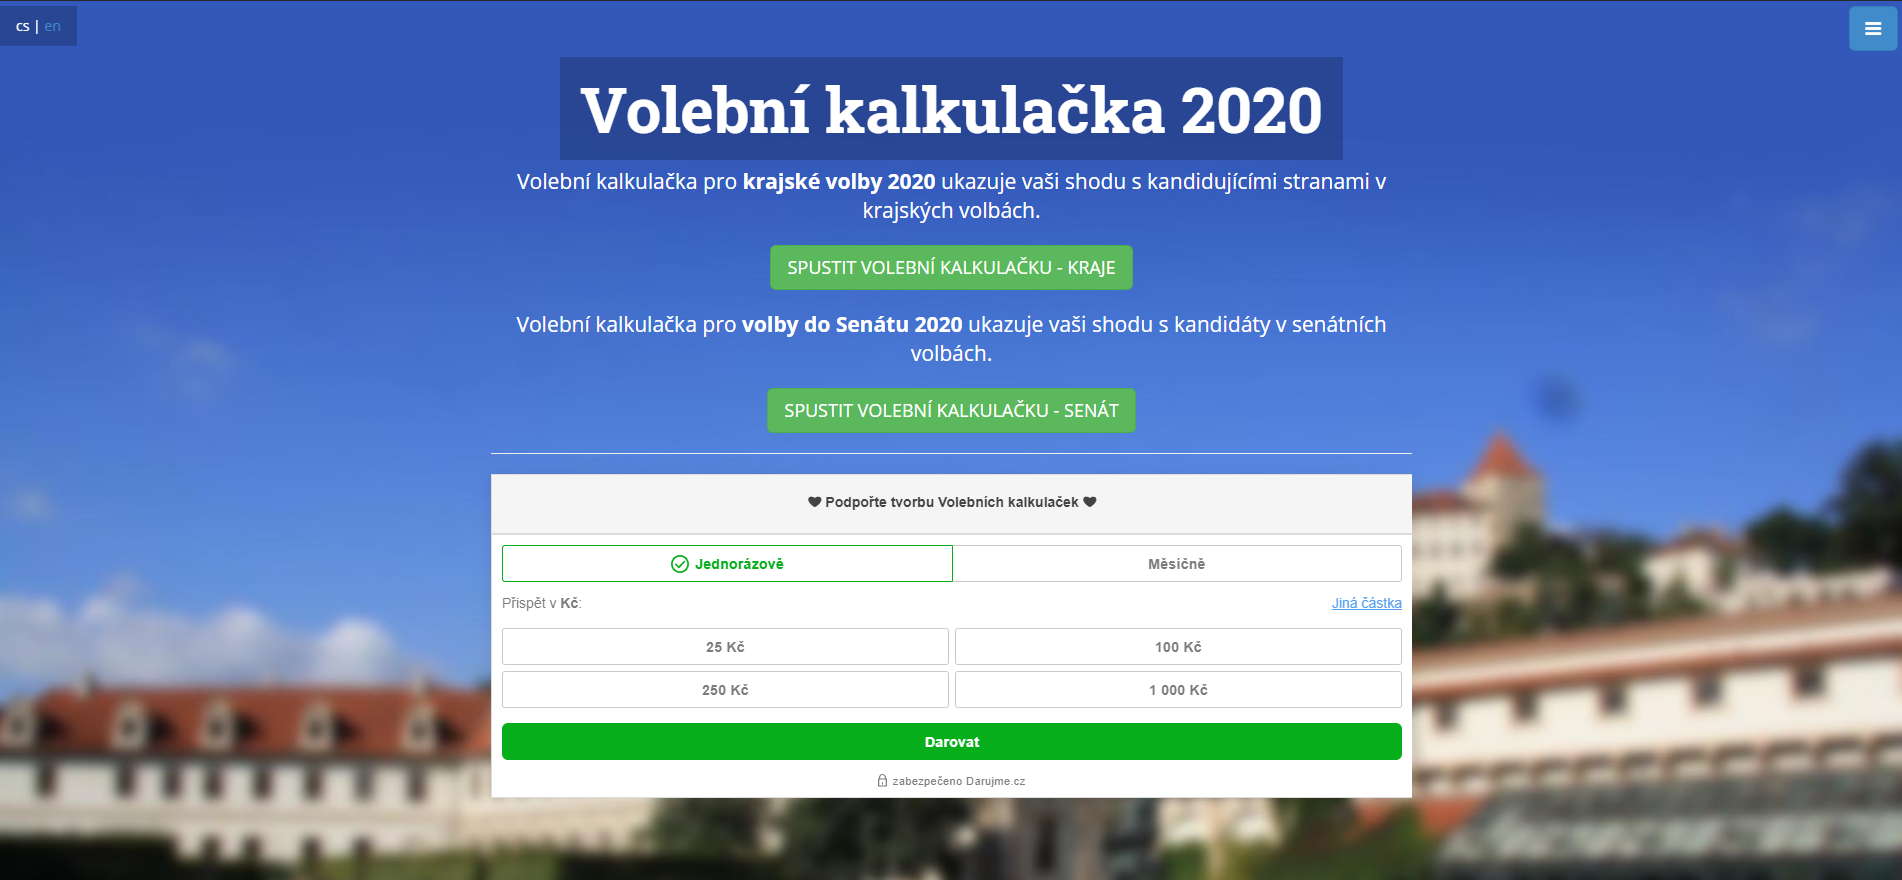
\includegraphics[width=1\textwidth]{obrazky-figures/volebnikalkulackacz-uvod.png}
    \caption{Úvodní stránka aplikace volebnikalkulacka.cz}
    \label{fig:volebnikalkulacka-uvod}
\end{figure}

\begin{figure}
    \centering
    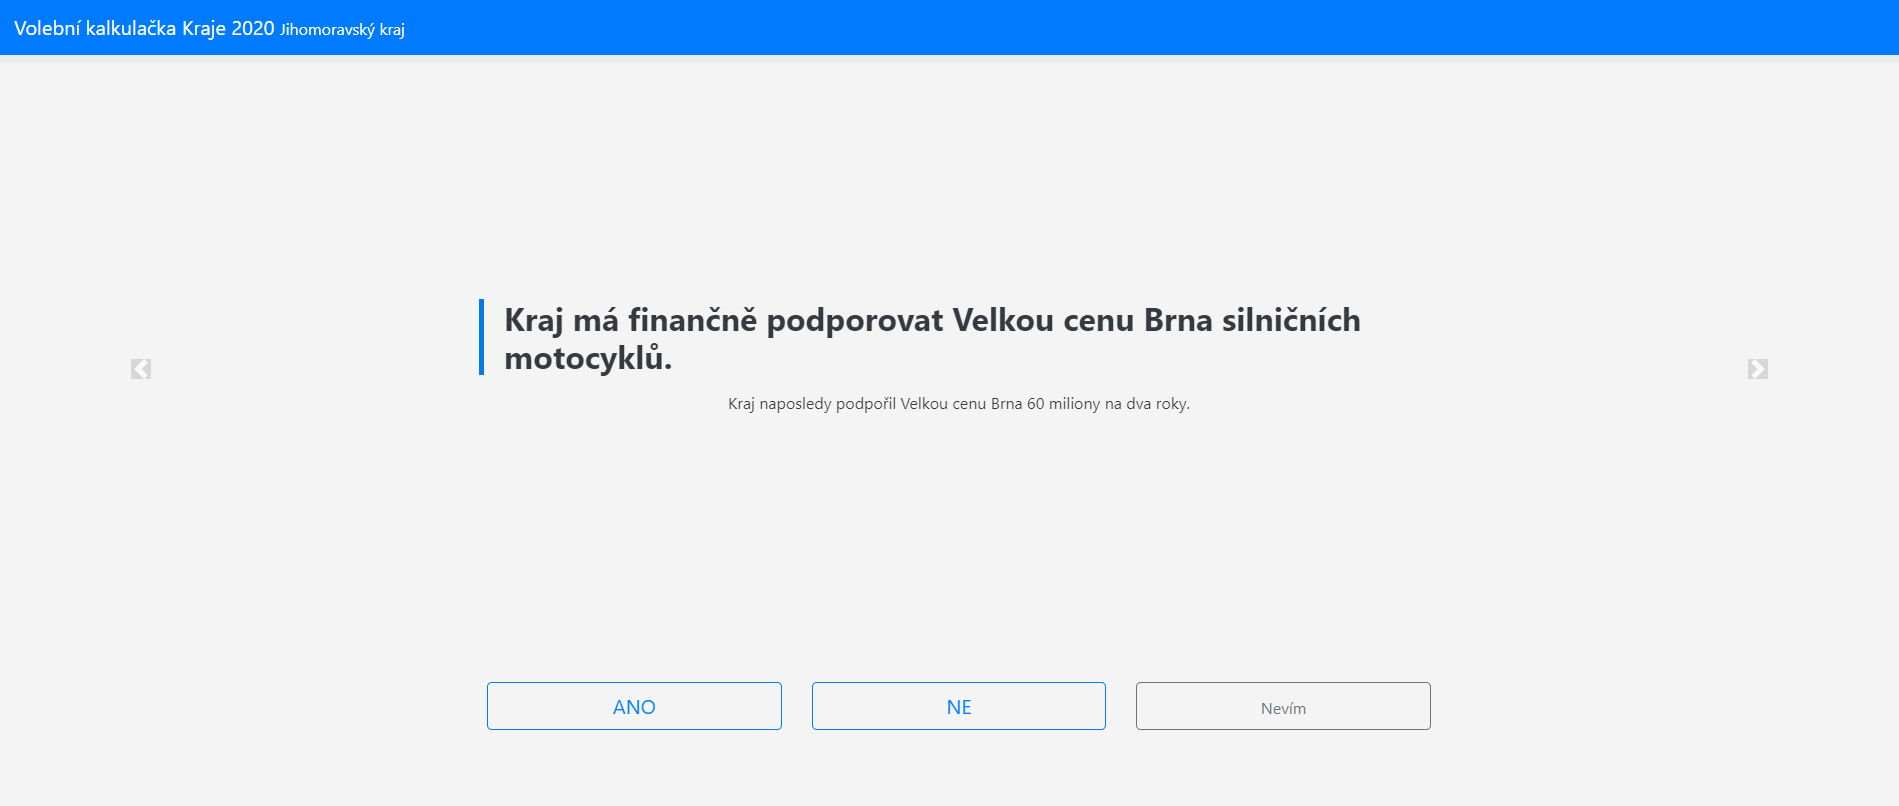
\includegraphics[width=1\textwidth]{obrazky-figures/volebnikalkulacka-otazka.png}
    \caption{Příklad otázky v aplikaci volebnikalkulacka.cz}
    \label{fig:volebnikalkulacka-otazka}
\end{figure}

\begin{figure}
    \centering
    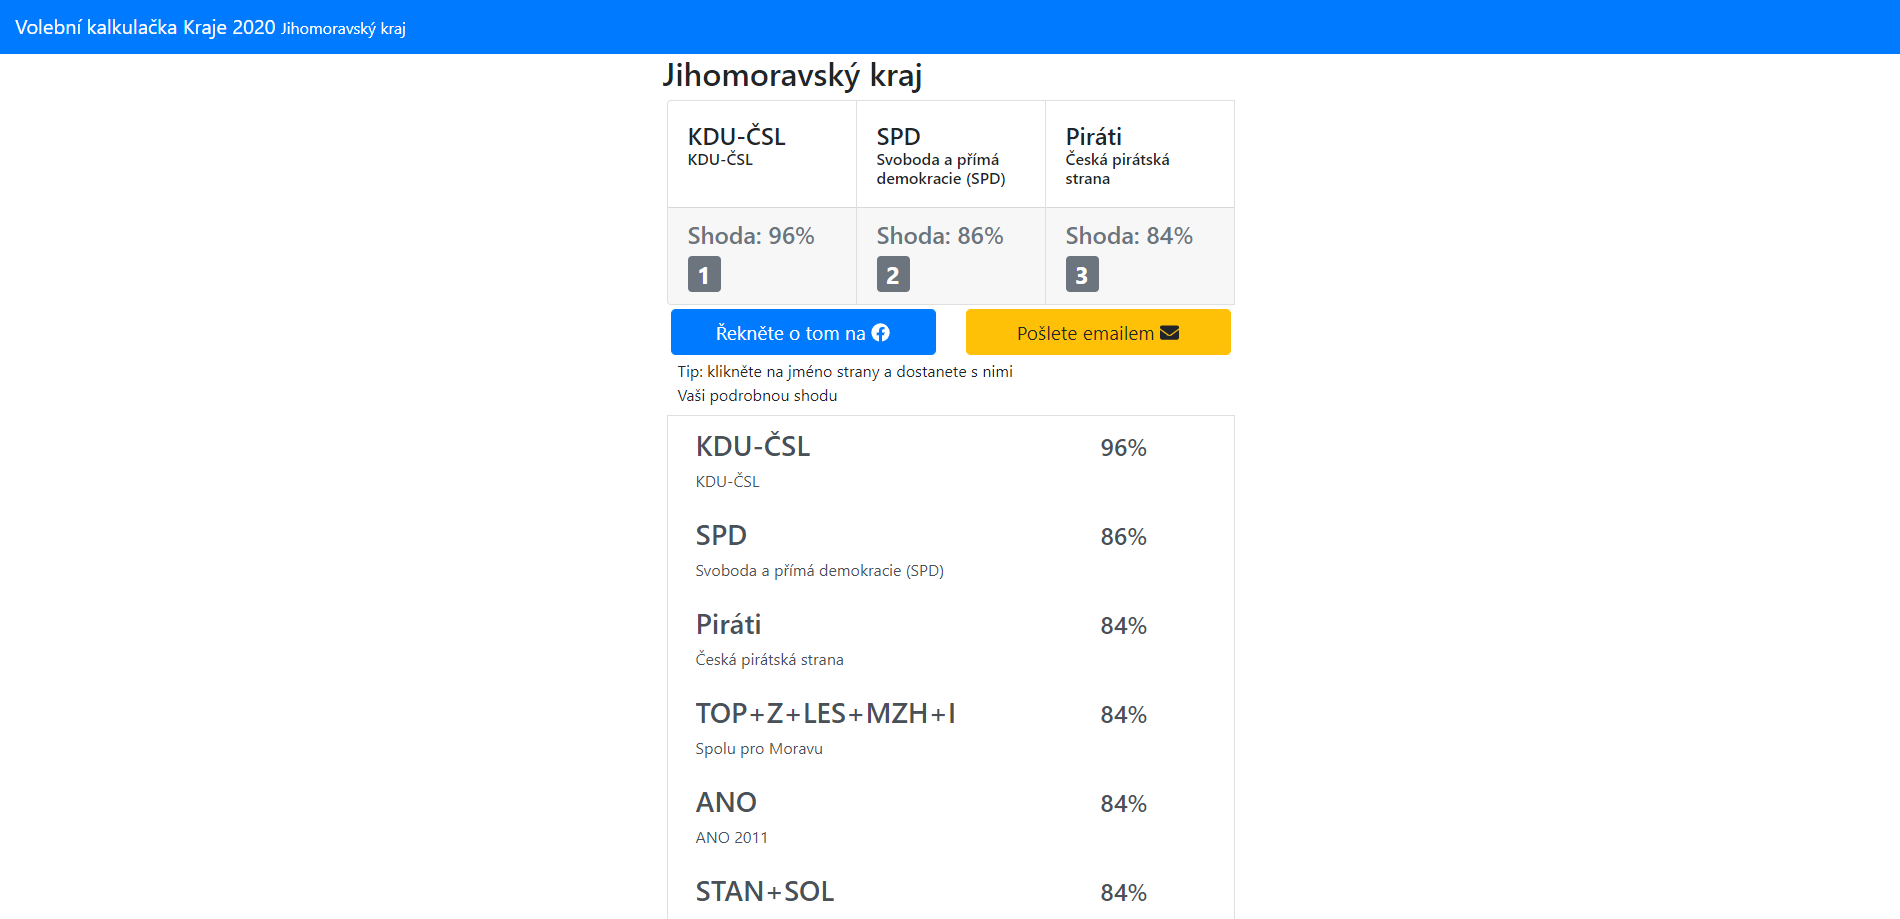
\includegraphics[width=1\textwidth]{obrazky-figures/volebnikalkulacka-vysledky.png}
    \caption{Příklad prezentace výsledků uživateli v aplikaci volebnikalkulacka.cz}
    \label{fig:volebnikalkulacka-vysledky}
\end{figure}




\subsection{iDnes.cz}
Princip této aplikace je totožný jako u volebnikalkulacka.cz. Liší se pouze některé otázky a grafický vzhled, který je zde přizpůsoben celkovému stylu zpravodajského webu idnes.cz,\footnote{idnes.cz: \url{https://www.idnes.cz/}} viz obrázek \ref{fig:idnes-uvod}. Dokonce mají obě aplikace i stejného autora, kterým je sdružení \mbox{kohovolit.eu}.\footnote{kohovolit.eu: \url{http://kohovolit.eu/}}

\begin{figure}
    \centering
    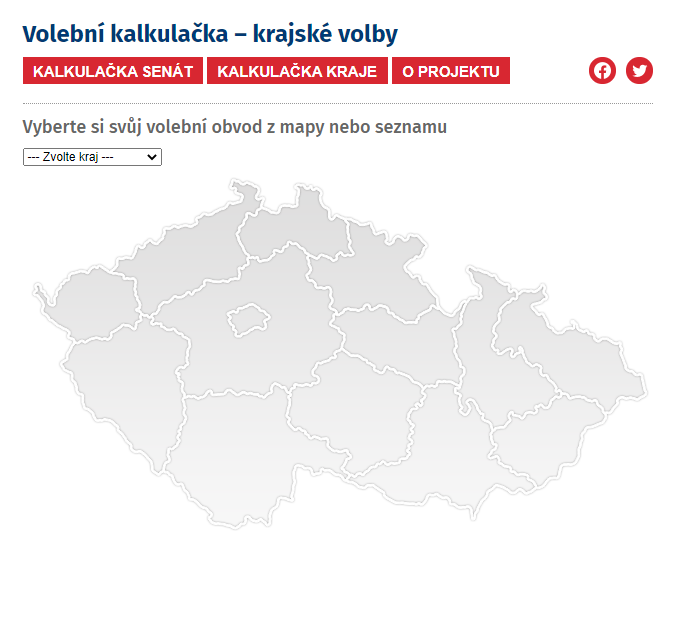
\includegraphics[width=0.7\textwidth]{obrazky-figures/idnes-uvod.png}
    \caption{Úvodní strana volební kalkulačky na webu Idnes.cz}
    \label{fig:idnes-uvod}
\end{figure}

\subsection{Postvolítko}
Přestože nejde o volební kalkulačku, je tato studentská aplikace velmi zajímavý nástroj pro zkoumání dat z Poslanecké sněmovny. Ta jsou zde přehledně a srozumitelně rozřazena do 3 různých přehledů - hlasování, poslanci a strany, jak můžeme vidět na obrázku \ref{fig:postvolitko-uvod}.

\begin{figure}
    \centering
    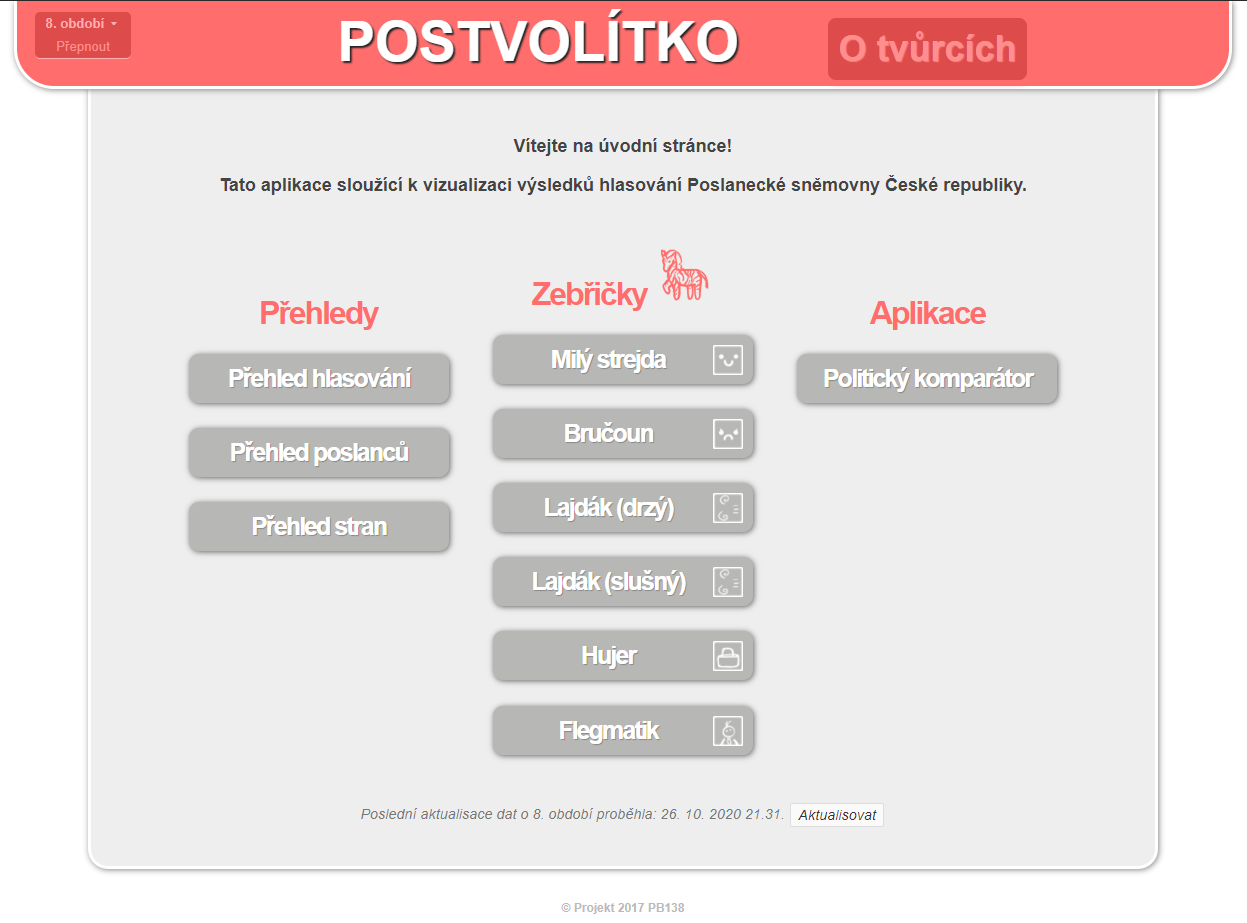
\includegraphics[width=0.7\textwidth]{obrazky-figures/postvolitko-uvod.png}
    \caption{Úvodní strana webové aplikace Postvolítko}
    \label{fig:postvolitko-uvod}
\end{figure}


\par Přehled hlasování nabízí výčet všech poslaneckých schůzí ve zvoleném volebním období. Tyto schůze jsou dále doplněny o přehled jednacích bodů schůze a k nim náležejících hlasování, obr. \ref{fig:postvolitko-hlasovani}. \\
U jednotlivých hlasování lze dále otevřít detail s konkrétními jmény poslanců a jejich volbou.

\begin{figure}
    \centering
    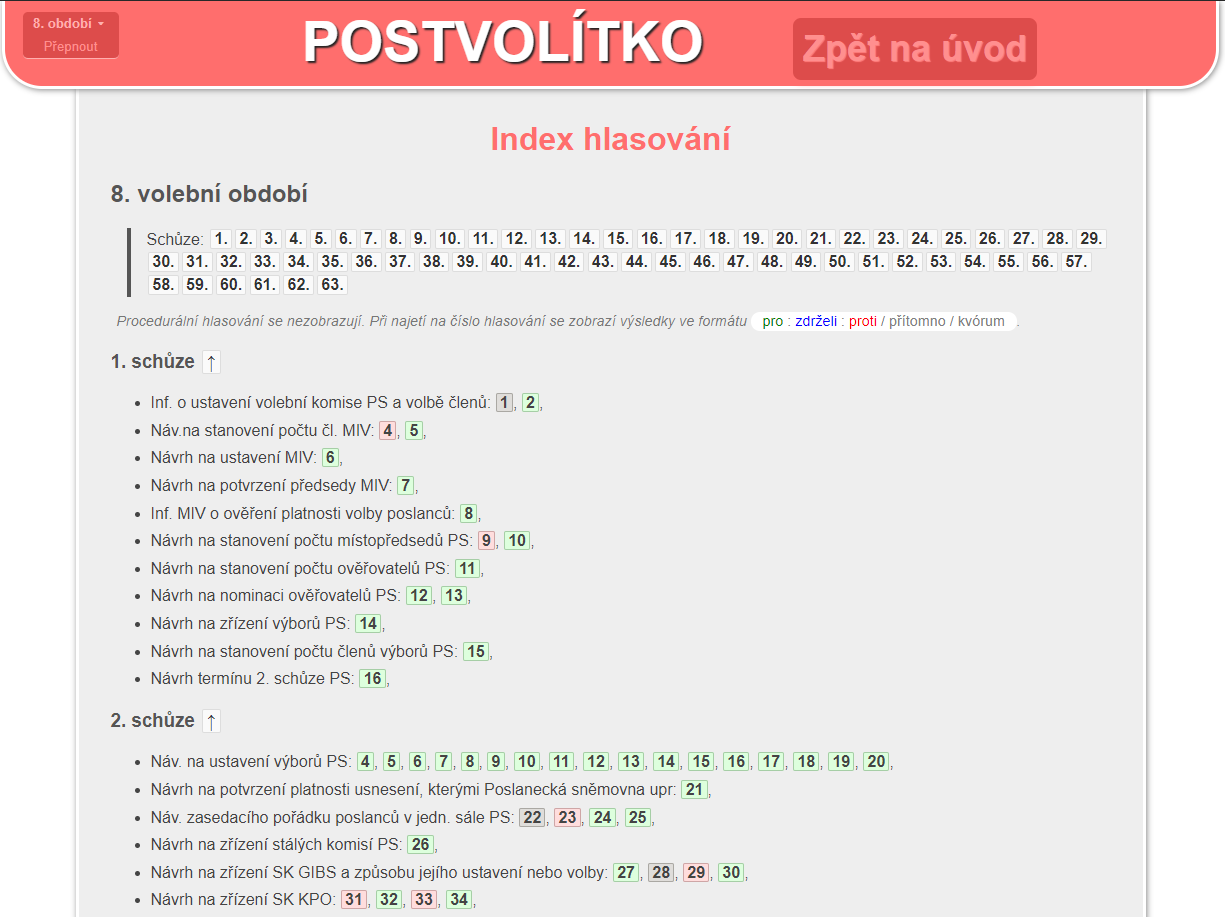
\includegraphics[width=0.7\textwidth]{obrazky-figures/postvolitko-hlasovani.png}
    \caption{Přehled schůzí a hlasování PS v aplikaci Postvolítko}
    \label{fig:postvolitko-hlasovani}
\end{figure}

\par Přehled poslanců nabízí seznam všech aktivních poslanců ve zvoleném volebním období. Pod jménem poslance se dále lze dostat na detail jeho osoby, kde nalezneme kromě jeho veřejně dostupných osobních údajů také statistiky jeho hlasování a absencí.


\par V přehledu stran nalezneme seznam všech aktuálně zúčastněnch stran v poslanecké sněmovně. Přes jednotlivé strany se dá opět dostat na jejich detail. Zde je opět seznam poslanců, pouze omezen na členy konkrétní strany.

\par Dále zde nalezneme žebříčky podle různých statistik, například podle počtu hlasování pro, počtu neomluvených hodin, či nejnižší absence. 
\par Poslední funkcí Postvolítka je porovnávání dvou vybraných poslanců a zobrazení jejich procentuální shody, vycházející ze stejných voleb u jednotlivých hlasování.


\section{Výchozí data}
Data, ze kterých tato práce čerpá, se nachází na oficiálním webu Poslanecké sněmovny Parlamentu České republiky\footnote{Oficiální web Poslanecké sněmovny: \url{https://www.psp.cz/sqw/hp.sqw}}. Konkrétně se jedná o data agend Poslanecké sněmovny\footnote{Data agend Poslanecké sněmovny: \url{https://www.psp.cz/sqw/hp.sqw?k=1300}}, poskytovaná veřejnosti zdarma pod podmínkou uvedení zdroje a data zpracování\cite{pspData}.
\par Zde dostupné záznamy popisují všechny schůze Poslanecké sněmovny až do roku 1993. Ty jsou dále děleny na popis samotné schůze a jejího stavu, jednotlivé body pořadu, jejich popis, stav a výsledek. Kromě samotných schůzí jsou k dispozici také záznamy o všech poslancích v tomto volebním období - fotky, pracovní emaily a telefony, ostatní funkce které vykonávají, či jejich hlasování a absence.
\par Data jsou strukturována v tabulkách, mezi nimiž jsou vzájemné vazby. Na obrázku \ref{fig:psp-tabulka-priklad} je struktura jedné z databázových tabulek. Ty nejpodstatnější vazby mezi tabulkami pro tuto práci jsou naznačeny na obrázku \ref{fig:psp-data-diagram}.
\par Jednou denně jsou všechna data aktualizována a doplněna o nové záznamy. Tato aktualizace probíhá v noci.



\begin{figure}
    \centering
    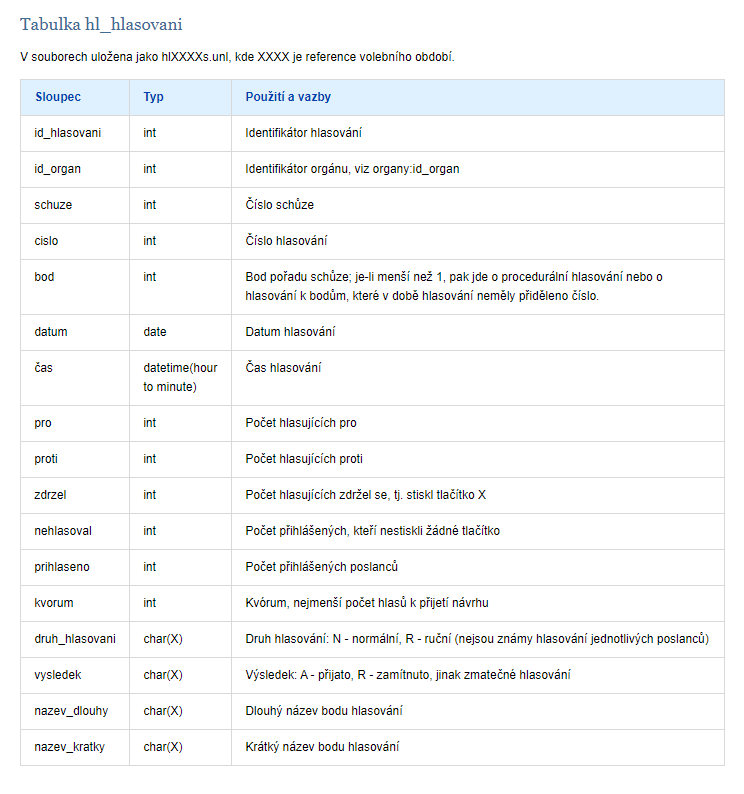
\includegraphics[width=0.8\textwidth]{obrazky-figures/psp-tabulka-priklad.png}
    \caption{Popis struktury jedné z datových tabulek Poslanecké sněmovny\cite{pspData}}
    \label{fig:psp-tabulka-priklad}
\end{figure}

\begin{figure}
    \centering
    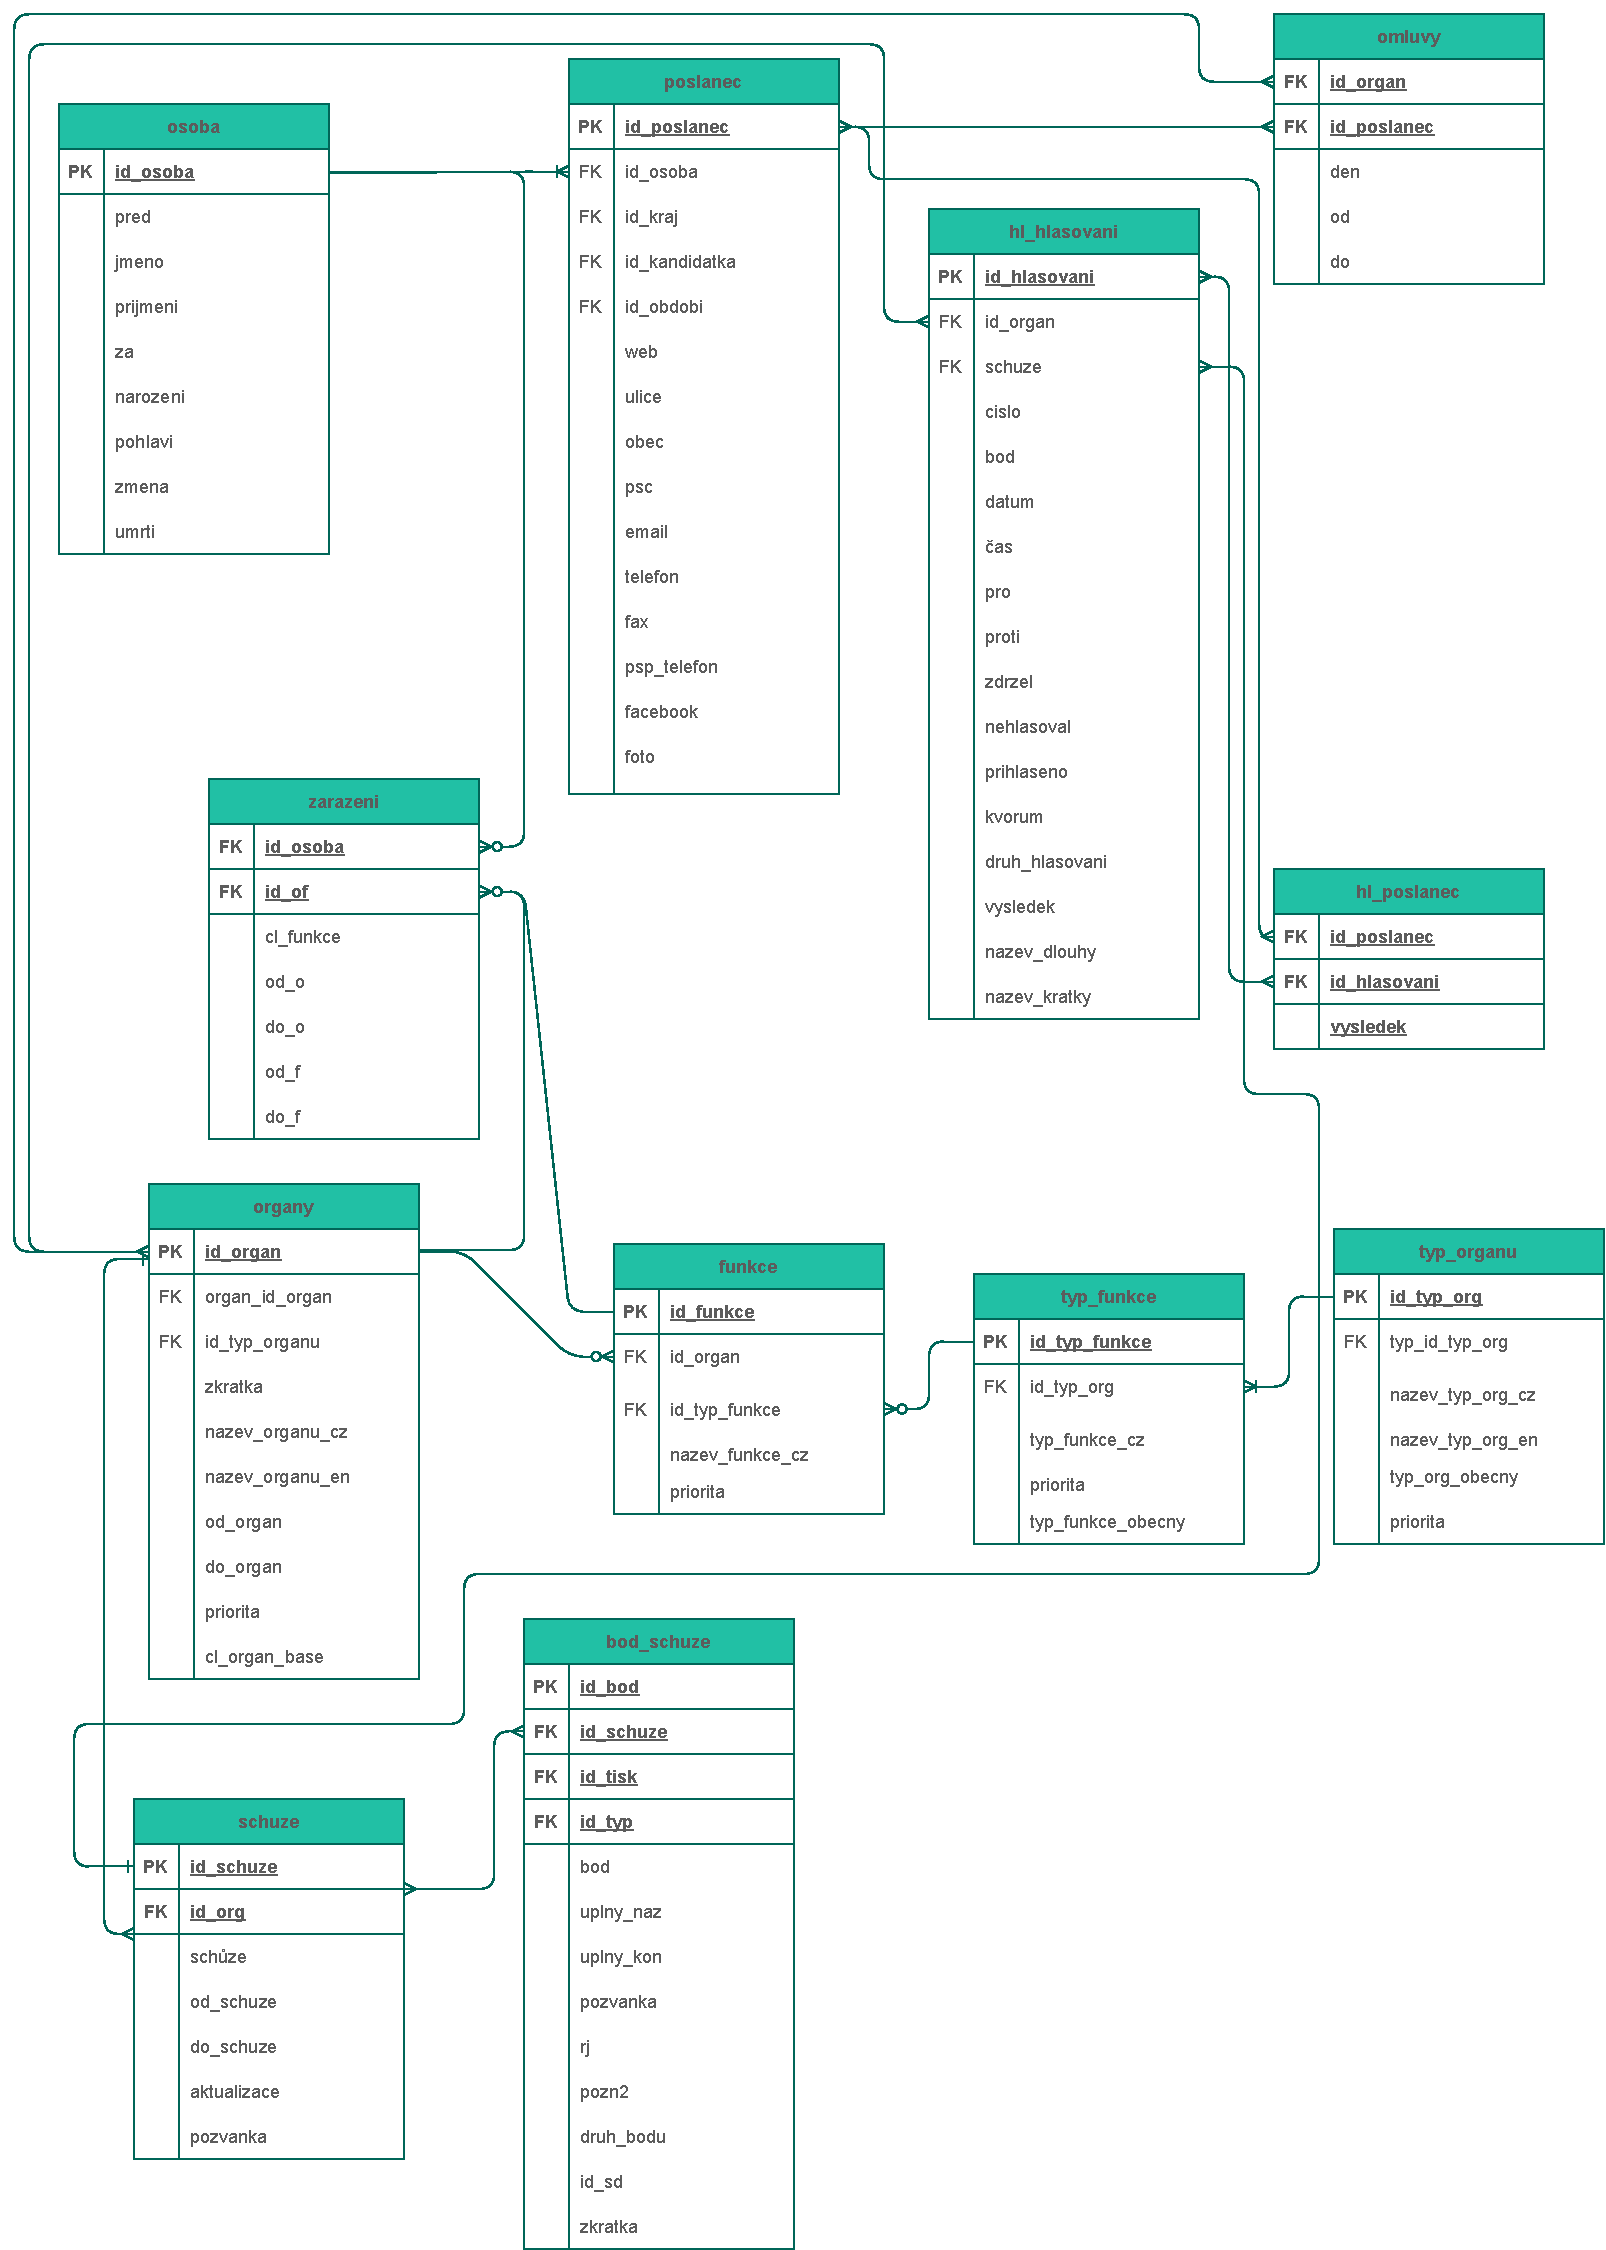
\includegraphics[width=1\textwidth]{obrazky-figures/data_diagramy.pdf}
    \caption{Diagram znázorňující vztahy některých datových tabulek}
    \label{fig:psp-data-diagram}
\end{figure}




%%%%%%%%%%%%%%%%%%%%%%%%%% TECHNOLOGIE  %%%%%%%%%%%%%%%%%%%%%%%%%%%%%%%
\chapter{Použité technologie}
\label{chap:technologie}
V této kapitole jsou stručně popsány použité technologie. Jedná se o webovou stránku, proto jsou na úvod představeny základní techniky k vytvoření statického webu. Po nich následuje představení technologií zajišťujících dynamičnost. Zde patří python a jeho framework Django.
\par Kapitola je zakončena popisem použitého databázového systému PostgreSQL.


\section{HTML, CSS}
HTML je zkratka pro \texttt{hyper text markup language}. Jak už název napovídá, tento jazyk není programovací, nýbrž strukturovací (značkovací). To znamená, že pomocí něj dokážeme vytvořit strukturu a význam částí dokumentu, který následně dokáží správně zobrazit a interpretovat webové prohlížeče. Často se přirovnává ke kostře lidského těla.  \cite{HTML}

\par CSS je zkratkou pro \texttt{cascading style sheets} a definuje jak budou HTML elementy zobrazeny. V překladu název znamená "kaskádové styly", kdy kaskádě odpovídá vrstvení jednotlivých stylů na sebe, ovšem vždy platí ten poslední, případně ten nejspecifičtější. Při použití předchozího přirovnání by CSS bylo jako maso a kůže. \cite{CSS} 


\section{Bootstrap}
Bootstrap\footnote{Bootstrap: \url{https://getbootstrap.com/}} je aktuálně nejpoužívanější CSS framework pro vývoj responsivních a tzv. \texttt{mobile-first} stránek. \cite{BOOTSTRAP} Poskytuje předpřipravené HTML a CSS komponenty, pomocí kterých se dá rychle a jednoduše vytvořit design webu. Klíčovým aspektem je využívání tříd, kterými je vývojář schopen jednoduše přiřadit HTML elementům styly, které bootstrap již v základu poskytuje, aniž by při tom musel neustále přecházet mezi HTML šablonou a CSS dokumentem. Jednou z nejvyužívanějších funkcí bootstrapu je možnost virtuálního rozdělení obsahu elementu na 12 stejných sloupců, se kterými lze pak jednoduše pracovat pomocí přidávání tříd na elementy obsahu. Velkou výhodou je také jednoduchá práce s responsivitou, opět pomocí různých tříd.
\par  Obecně existují dva způsoby myšlení při vytváření webové stránky. První je navrhnout nejprve verzi pro stolní počítače, respespektive celkově velké obrazovky a pak ji postupně obírat o funkcionalitu, aby byla použitelná i na telefonu. Tento způsob byl přijatelný dříve, kdy mobilní telefony sloužily primárně k telefonování a počet návštěvníků webu z nich nebyl nijak závratný. Se zvyšujícím se využitím mobilních telefonů pro prohlížení internetu, kdy v dnešní době více než polovina lidí tzv. "surfuje" na telefonu \cite{WEB-DEVICE-USAGE}, je však již považován za nedostatečný.
\par Tím druhým je právě \texttt{mobile first}, kdy se nejprve navrhne design pro mobilní telefony a až s přibývajícím místem na obrazovce se doplňují i pokročilejší designové prvky a funkce. Tento způsob je obecně využívanější, jelikož je pro vývojáře ve většině případů mnohem komfortnější a zaměřuje se primárně na jednoduchost a ovladatelnost právě na malých obrazovkách, kde to mnohdy může být pro uživatele problém.

\section{Sass}
Sass\footnote{Sass: \url{https://sass-lang.com/}} je jeden z několika běžně používaných CSS preprocesorů.\footnote{CSS preprocesory: \url{https://raygun.com/blog/css-preprocessors-examples/}} Ve své podstatě je CSS preprocesor nástroj, respektive jazyk, který zjednodušuje, zpřehledňuje a zrychluje stylování webových stránek. Snaží se zvýšit efektivitu psaní kódu pomocí minimalizace nutnosti kopírovat velké bloky již jednou napsaného kódu, což je konkrétně u CSS běžná věc. Přidává například možnost použití proměnných, zanořování selektorů, využívání mixinů. 
\par Prohlížeče nicméně stále ještě pracují pouze s čistým CSS, proto se do něj jazyk preprocesorů musí překládat před tím, než ho server odešle uživateli. 


\section{JavaScript}
JavaScript\footnote{JavaScript: \url{https://developer.mozilla.org/en-US/docs/Web/JavaScript}} je scriptovací jazyk umožňující dynamicky měnit obsah stránky bez nutnosti stránku znovu načíst. Kromě toho umí také spoustu dalších věcí, kupříkladu ovládat multimédia a animovat jednotlivé elementy. Naprostá většina moderních prohlížečů má jeho podporu již vestavěnou, mezi výjimky patří například textový prohlížeč Lynx\footnote{Lynx: \url{https://lynx.browser.org/}}. Podle dostupných statistik \cite{JAVASCRIPT-USAGE} je dnes JavaScript využíván na 95\% webových stránek.

\section{jQuery}
jQuery\footnote{jQuery: \url{https://jquery.com/}} je malá knihovna určená ke zjednodušení práce s JavaScriptem. Hlavní snahou je zmenšení množství napsaného kódu, nutného k vytvoření požadované funkcionality, spolu se zjednodušením používání některých JavaScriptových prvků, kupříkladu AJAX volání. \cite{JQUERY} Další z výhod jQuery je obrovské množství dostupných pluginů, díky kterému je často možné jednoduše odstranit i komplikované problémy pomocí již hotového řešení.\footnote{jQuery pluginy: \url{https://plugins.jquery.com/chosen/}}  
\par jQuery je v současné době nejspíše nejpopulárnější JavaScriptový framework, využívaný na více než 19 milionech webových stránek \cite{JQUERY-USAGE}. Najdeme ho obsažen také v populárním systému správy obsahu Wordpress\footnote{Wordpress: \url{https://wordpress.org/}}.

\section{Python}
"Python\footnote{Python: \url{https://www.python.org/}} je interpretovaný, objektově orientovaný, vysokoúrovňový programovací jazyk s dynamickou sémantikou." \cite{PYTHON} \\
Kromě toho je v současné době asi nejrychleji rostoucím a nejoblíbenějším programovacím jazykem napříč celou škálou oborů, díky své jednoduchosti a intuitivnosti. Využívá se ve všech možných aplikacích, od základní automatizace opakujících se činností, například zpracování excelu, nebo zpracování dat z webových stránek, přes matematické analýzy, analýzu a vizualizaci dat, až po vytváření umělé inteligence. Mimo to ho lze využít také k vytváření aplikací, mobilních, desktopových i webových. Právě kvůli možnosti vytvoření webové aplikace, která bude zároveň mít možnost zpracovávat a analyzovat data bez nutnosti přidávání dalších nástrojů, byl jazyk python zvolen pro backend této práce.

\section{Django}
Django\footnote{Django: \url{https://www.djangoproject.com/}} je volně dostupný, open-source framework pro webové aplikace napsané v jazyce Python. Jeho smyslem je ulehčit a urychlit vytváření webových aplikací. Za tímto účelem poskytuje již předpřipravenou strukturu, zajišťující například zabezpečení, práci s databází, šablonování, autentizaci a jiné. Django vychází z návrhového vzoru MVC, kde \texttt{Controller} je nahrazen šablonami (anglicky "Template"), tedy \texttt{MVT}. Kromě toho Django obsahuje množství volně dostupných pluginů rozšiřujících jeho funkcionalitu. Nechybí také přehledná a rozsáhlá dokumentace.


\section{PostgreSQL}
PostgreSQL\footnote{PostgreSQL: \url{https://www.postgresql.org/}} je výkonný objektově-relační, open-source, databázový systém využívající a zároveň rozšiřující jazyk SQL. Jeho vznik se datuje až do roku 1986 a za dobu své existence si získalo pověst spolehlivého, robustního a jednoduše rozšiřitelného řešení databáze. \cite{PostgreSQL}
\par Při volbě databázového systému byl původní kandidát MySQL, jelikož s ním často pracuji a všechno potřebné jsem tak měl již připravené. Nicméně podle některých názorů \cite{WHY-POSTGRES1}\cite{WHY-POSTGRES2} je obecně lepší využívat databázový systém PostgreSQL, jelikož je na něj Django lépe připravené a používají ho i sami vývojáři, takže bude lépe dokumentován.



%%%%%%%%%%%%%%%%%%%%%%%%%% Návrh %%%%%%%%%%%%%%%%%%%%%%%%%%%%%%%
\chapter{Návrh aplikace}
\label{chap:navrh}
U webových aplikací obecně platí, že rozhodnutí uživatele o využití či opuštění stránky z velké části závisí na designu a použitelnosti. Proto je třeba, aby kromě kvalitní funkcionality měla aplikace také moderní a promyšlený vzhled. \\
Nejprve je třeba vytyčit cílovou skupinu. Díky tomu zjistíme, na jaké části systému je třeba se zaměřit a případně jakým způsobem je nejlépe zpracovat pro co největší uživatelský komfort. Dalším krokem je analýza případů užití, pomocí které zjistíme, jaké funkce budou uživatelé používat. Následuje návrh databáze, vycházející z dat, se kterými chceme pracovat a z jejich vztahů. Kapitola vrcholí samotným grafickým návrhem, zpracovávajícím všechny předchozí kroky do jednoho úhledného a intuitivního uživatelského rozhraní.


\section{Cílová skupina}
Cílová skupina kalkulačky budou obecně všichni lidé s volebním právem, tedy občané České republiky starší 18-ti let.\cite{ustava-volebni_pravo} Podle statistiky zveřejněné na webu statistikaamy.cz\footnote{statistikaamy.cz: \url{www.statistikaamy.cz}}, který spravuje Český statistický úřad\footnote{Český statistický úřad: \url{https://www.czso.cz/csu/czso/domov}}, používalo v roce 2016 internet 32,5\% z lidí starších 65 let\cite{statistikaamy}. Bude tedy třeba zvýšit důraz na jednoduchost, přehlednost a intuitivnost, které jsou zejména pro starší lidi kritické.
\par Dále lze tuto skupinu rozdělit na dvě menší části. Tou první jsou lidé, kteří využíjí naplno všech funkcí webu, včetně registrace a uložení výsledků na svůj profil. Zde budou spadat zejména mladší uživatelé. Pro ty bude důležité, aby registrace byla jednoduchá a rychlá a zároveň jim web umožňoval spravovat svůj profil a své uložené výsledky. Pro ty nejmladší bude také podstatné mít možnost jednoduše sdílet své výsledky na sociální sítě.
\par Zbylá část bude tvořena lidmi, které bude zajímat pouze jejich výsledek a hned po jeho zjištění web opustí. V tomto případě je nutné co nejvíce zjednodušit přístup k hlavní funkční části webu.


\section{Případy užití}
Po příchodu na web uvidí každý uživatel domovskou stránku, poskytující základní přehled o smyslu a cíli aplikace. Na výběr zde má celkem tři akční oblasti. Kromě horního menu a patičky, které jsou přístupny na každé stránce aplikace, také velké akční tlačítko sloužící pro přechod do kalkulačky. Použití kalkulačky je pro všechny uživatele stejné, liší se až konec, kdy registrovaný a přihlášený uživatel může využít možnosti uložit si právě získané výsledky ke svému profilu. Každý uživatel může také své výsledky sdílet na sociálních sítích. 
\par Horní menu odkazuje na jednotlivé části aplikace, na přehledy poslanců, hlasování a stran, které může použít každý uživatel. Je zde také tlačítko pro přihlášení, případně odkaz na uživatelský účet, pokud již uživatel přihlášený je. Pokud není, je mu přes něj umožněno se buď přihlásit, nebo přejít dalším odkazem na registrační formulář. Z přehledu poslanců se dá následně přejít na detail jednotlivých poslanců. Zde může registrovaný uživatel ohodnotit konkrétního poslance pomocí hvězdiček, či přidat komentář. Tyto dvě funkce byly omezeny pouze pro přihlášené uživatele z důvodu možného falšování hodnocení, či urážlivých komentářů. 
\par Přihlášeným uživatelům se přechodem do jejich účtu umožní upravovat svůj profil - přidat či upravit profilovou fotku, změnit heslo, spravovat svoje uložené výsledky.
\par V patičce pak má každý uživatel přístup k informacím o webu a ke stránce s kontakty.

\par
Případy užití znázorňuje diagram případů užití na obrázku \ref{fig:diagram_uc}

\begin{figure}
    \centering
    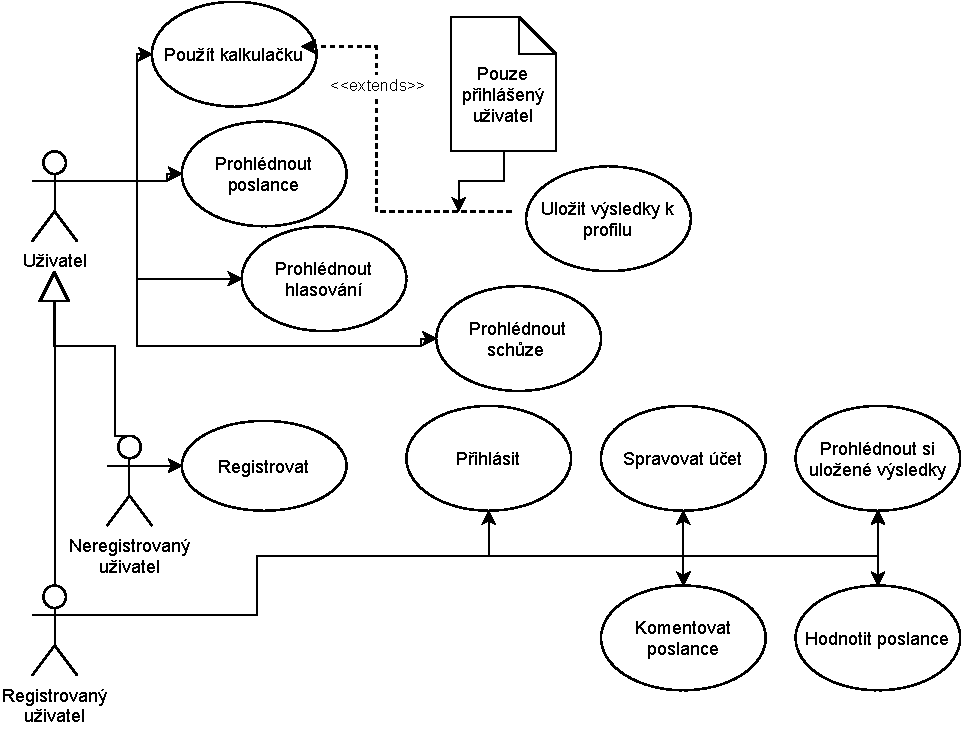
\includegraphics[width=0.8\textwidth]{obrazky-figures/UC.pdf}
    \caption{Diagram případů užití pro volební kalkulačku}
    \label{fig:diagram_uc}
\end{figure}



\section{Návrh databáze}
\todo{ER vygeneruje Django}\\


\section{Drátový model}
\label{section:wireframe}
Drátový, nebo-li takzvaně \texttt{wireframe} model, slouží ke zjednodušené vizualizaci umístění jednotlivých prvků webu v prostoru. Měl by obsahovat všechny elementy, které se budou na výsledném webu nacházet, nejlépe již i v konkrétních velikostech, aby šlo už v této fázi zjistit a odstranit případné nedostatky v rozložení. Smyslem tohoto modelu není zobrazit jak bude web vypadat, pouze jeho strukturu. Proto se používají spíše černobílé, či jednobarevné modely, ve kterých jsou designové bloky a obrázky nahrazeny jednoduchými obdélníky.
\par V ideálním případě se pro každý typ podstránky dělají až 4 drátové modely, v závislosti na různých typech responzivního zobrazení. V této práci postačuje jedna velikost, vytvořená v programu AdobeXD\footnote{AdobeXD: \url{https://www.adobe.com/products/xd.html}}. Jak vypadá drátěný model úvodní strany lze vidět na obrázku \ref{fig:wireframe-homepage}. Kompletní model je přiložen jako příloha \todo{Č. přílohy}. 

\begin{figure}
    \centering
    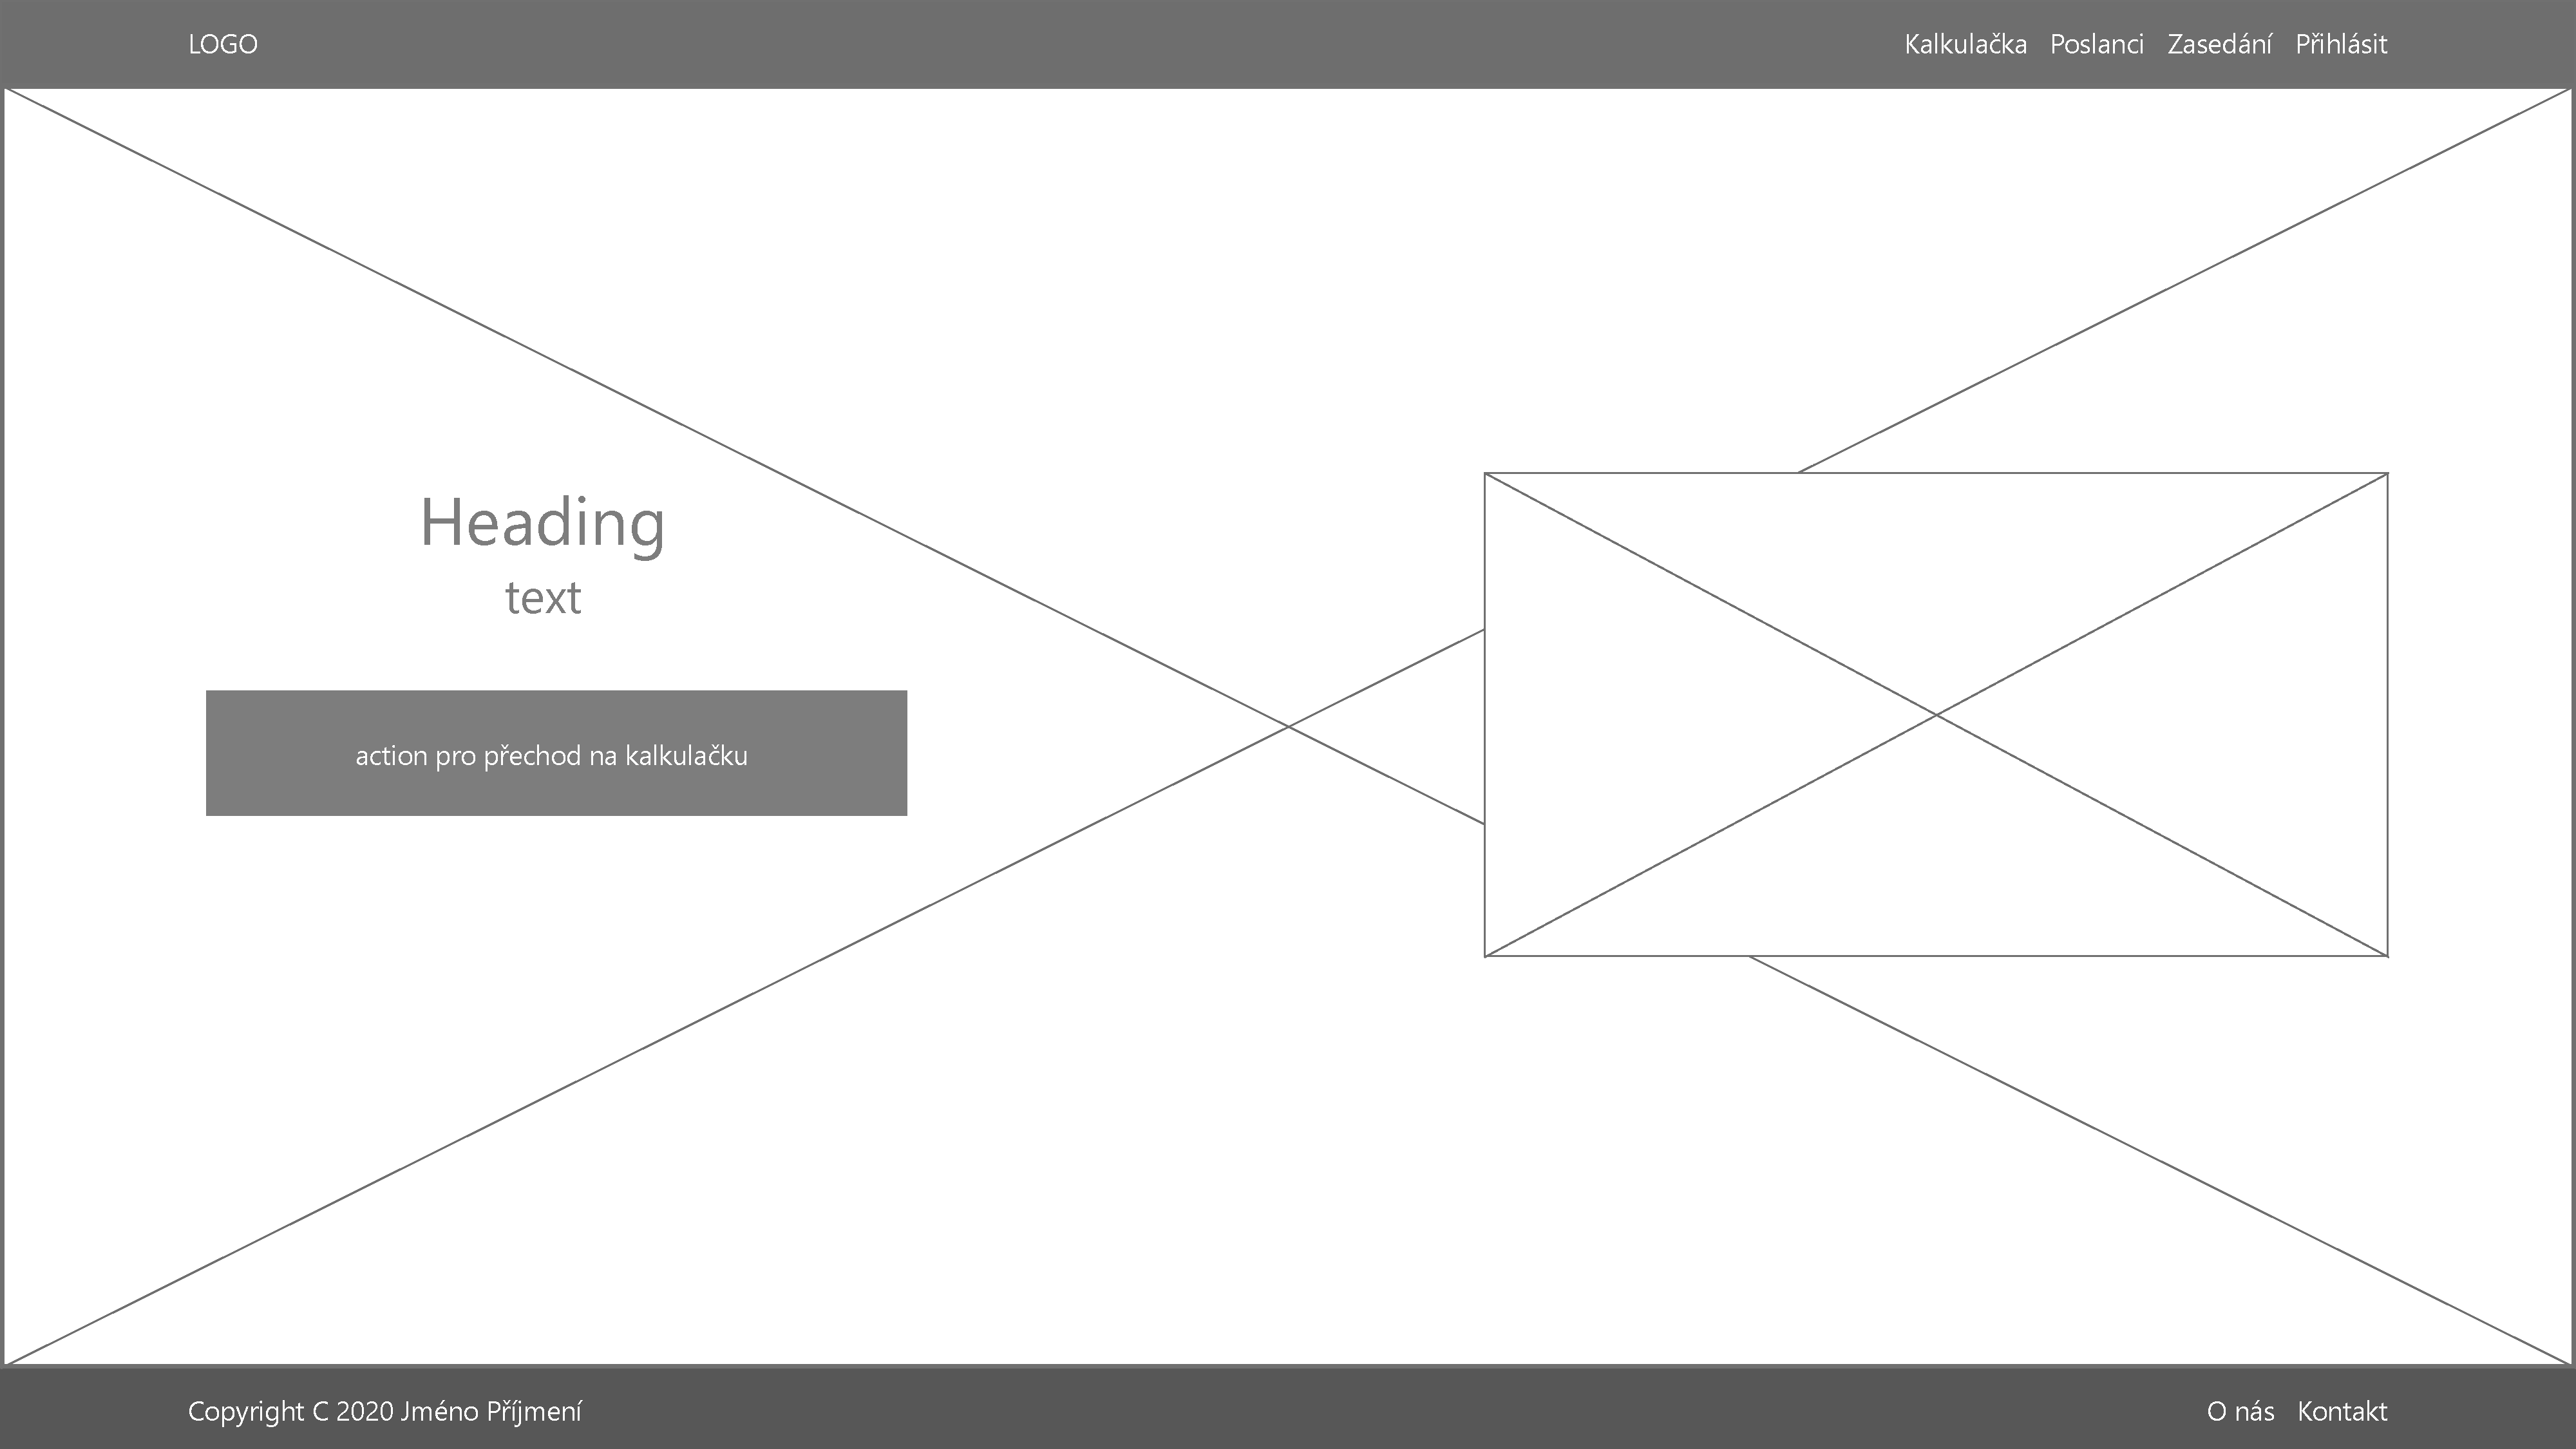
\includegraphics[width=0.8\textwidth]{obrazky-figures/wireframe-homepage.pdf}
    \caption{Drátěný model úvodní strany aplikace}
    \label{fig:wireframe-homepage}
\end{figure}



\section{Uživatelské rozhraní}
Při návrhu uživatelského rozhraní je obecně třeba dodržovat základy UX\footnote{UX: user experience} (česky \texttt{uživatelská zkušenost}) a UI\footnote{UI: user interface} (česky \texttt{uživatelské rozhraní}) designu. Tyto dva pojmy se v stále častěji zmiňují při tvorbě webových stránek a aplikací, nicméně nezřídka dochází k jejich zaměňování. 
\par UX design řeší, jakým způsobem bude uživatel s produktem pracovat. Tím obecně nemusí být myšlena jen digitální aplikace, ale může se jednat také o nějakou fyzickou věc, či službu. O cokoliv co může uživatel nějakým způsobem zažít. Do UX designu patří například drátový model, viz sekce \ref{section:wireframe}
\par Pokud jde o UI, tak na rozdíl od UX se jedná již o čistě digitální pojem. Uživatelské rozhraní je, zjednodušeně řečeno, místo, na kterém uživatel může komunikovat s aplikací. UI zahrnuje celkový vzhled, interaktivitu a intuitivnost aplikace a také celkový uživatelský pocit z používání. V současné době se zde řadí také responsivita.

\subsection{Postup při návrhu uživatelského rozhraní}
Jako první bylo třeba vypracovat základní strukturu webu se všemi prvky. K tomu posloužil již zmiňovaný drátový model. Tento byl po vytvoření prezentován nezainteresovaným lidem v roli uživatelů, aby byla získána zpětná vazba. Na jejím základě došlo k několika úpravám.
\par Jako další krok bylo potřeba vymyslet název a z něj vycházející logo celé aplikace. Jelikož smyslem celé práce je poskytnout lidem radu, čili učinit je chytřejšími (chytrý je anglicky \texttt{smart}), a následně jim díky tomu ulehčit výběr při volbě (anglicky \texttt{vote}), nabízelo se spojení právě těchto dvou slov. Původní volba byla SmartVote, nicméně po kontrole dostupnosti domény byla zvolena prohozená verze, čili VoteSmart, nebo-li česky \texttt{Volte chytře}. Samotné logo bylo následně vytvořeno ve webové aplikaci freelogodesign.org\footnote{freelogodesign.org: \url{https://www.freelogodesign.org/}}. Je tvořeno jménem webu a symbolem zaškrtávacího políčka, který je úzce spjat s účelem webu.
\par Následuje výběr vhodného barevného schématu. Jelikož se jedná o politicky orientovanou aplikaci pro prostředí České republiky, nabízí se použití národních barev - červené, modré a bílé. Konkrétní barevné hladiny (\#11457e pro modrou a \#d7141a pro červenou) byly převzaty z jedné z použitých grafik, konkrétně z mapy České republiky\cite{grafika-mapa}, viditelné na grafickém návrhu na úvodní straně. 
\par Jako font byl zvolen Segoe UI. Primární používané velikosti jsou 35px pro nadpisy H1, 25px pro H2 a 16px pro běžný text.
\par Samotný grafický návrh, viz příloha \todo{cislo prilohy} byl vypracováván opět v programu AdobeXD. Na obrázku \ref{fig:graphic-homepage} můžete vidět design úvodní strany. Při vytváření grafického návrhu byly použity principy responsivního designu, nicméně samotný návrh je pouze pro desktopovou\footnote{Desktopová verze je slangový výraz pro běžné obrazovky stolních počítačů, obecně s poměrem stran 16:9} verzi. 


\begin{figure}
    \centering
    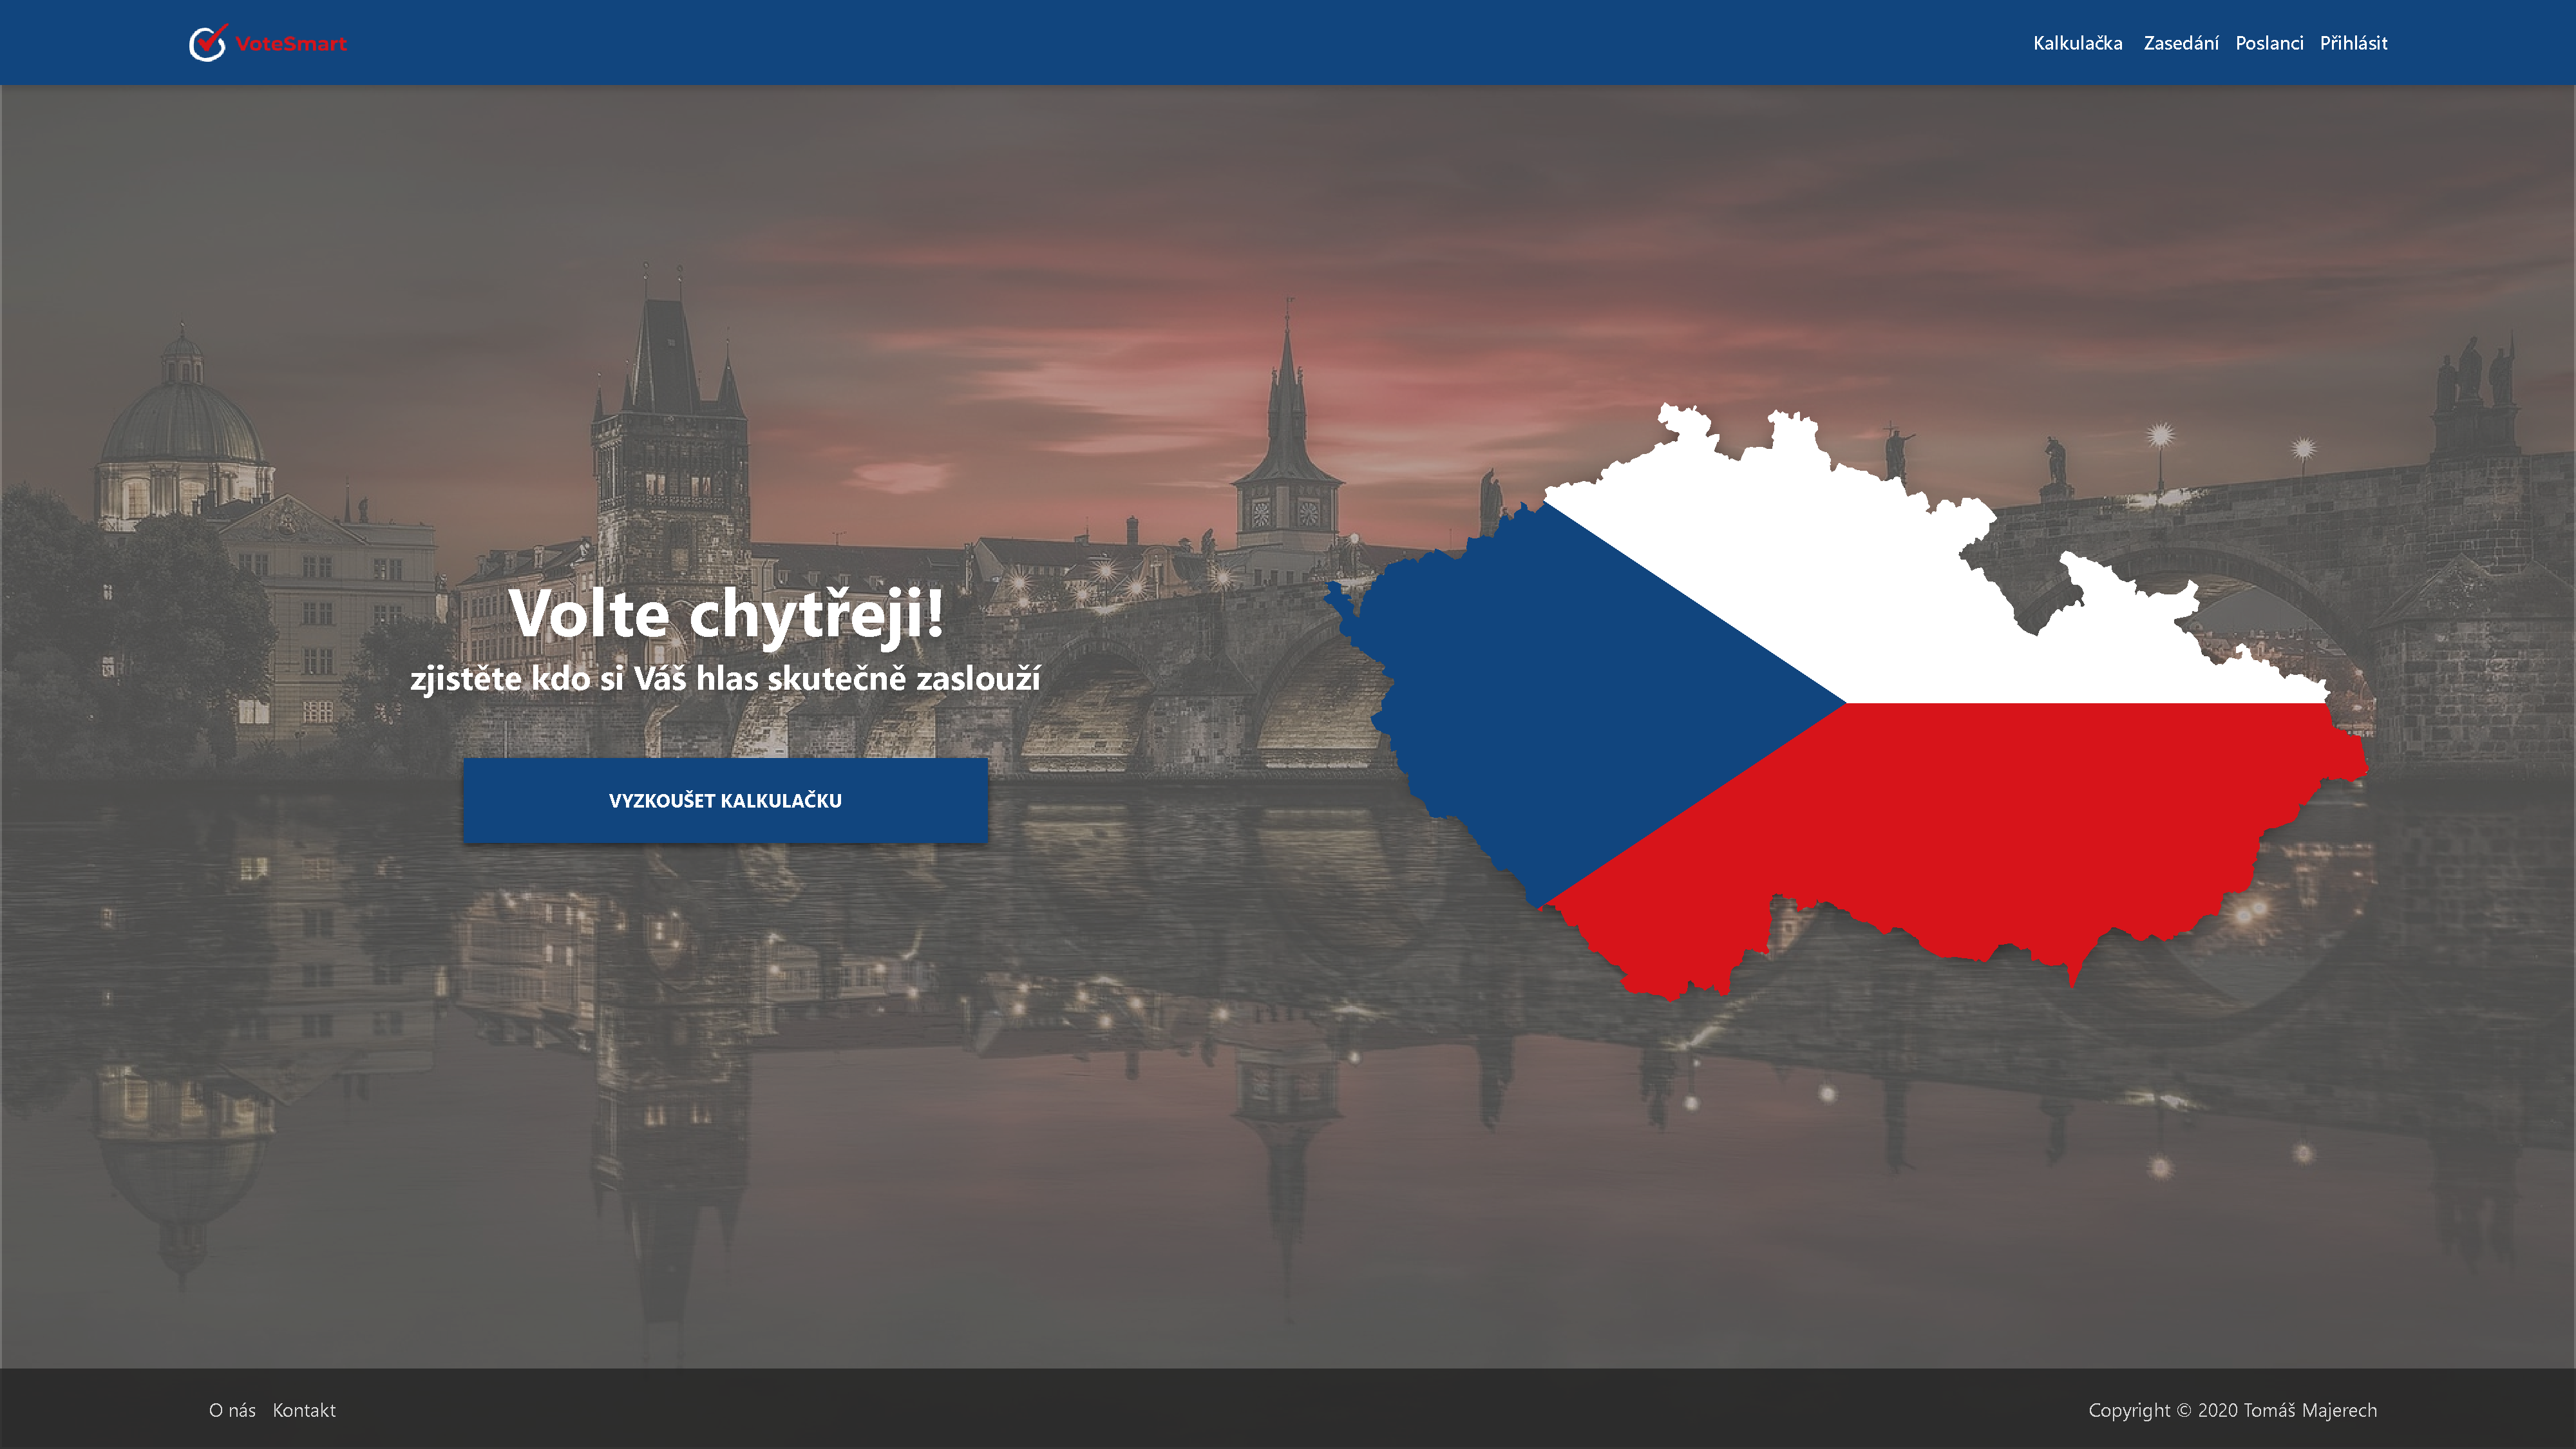
\includegraphics[width=0.8\textwidth]{obrazky-figures/Homepage.pdf}
    \caption{Grafický návrh úvodní strany aplikace}
    \label{fig:graphic-homepage}
\end{figure}

\todo{Možná rozvést jednotlivé strany?}

\section{Výběr otázek}
Jedná se o nejobtížnější a nejspíše také nejdůležitější část celé práce. Na výběru vhodných otázek totiž záleží nejenom to, nakolik dokážeme uživateli přiřadit podobnost s jednotlivými stranami a poslanci, ale také zda budou pro uživatele natolik zajímavé, aby vůbec použití kalkulačky dokončil.
\par Konkrétně z hlediska zajímavosti otázek není možné, aby byl jejich výběr plně automatizován, vždy bude na konci muset být člověk, který dokáže tento aspekt vyhodnotit. Nicméně vhodnou analýzou dat mu můžeme tento proces značně zjednodušit.
\par Jelikož pod pojmem otázka se v našem případě rozumí jedno ze skutečných hlasování, které v Poslanecké sněmovně proběhlo, mluvíme o výběru z tabulky \texttt{hl\_hlasovani}. Záznamů pro aktuální volební období je zde v době psaní této zprávy 7932. Nicméně většina z nich není pro naše účely důležitá, jelikož neměly vliv na výsledný stav návrhu, či byly pouze procedurální. Na první pohled však není možné rozhodující hlasování odlišit, musíme proto využít tabulky \texttt{hist} z balíčku dat sněmovních tisků. Ta uchovává údaje o projednávání každého sněmovního tisku a změně jeho stavů. Jelikož sněmovní tisky jsou podkladem pouze pro návrhy zákonů, můžeme tedy podle této tabulky vybrat pouze ty a všechno ostatní odfiltrovat. Tímto dokážeme zredukovat potenciální kandidáty na necelých 500.\\

\par V tomto bodě se dále nabízí možnost filtrovat podle sloupce \texttt{id\_prechod} v tabulce \texttt{hist}, přes který jsme schopni zjistit do jaké fáze legislativního procesu tisk a tedy i návrh po hlasování vstupuje. Toho dosáhneme spojením přes tento sloupec s tabulkou \texttt{prechody} a následným dalším spojením zde přes sloupec \texttt{kam} do tabulky \texttt{stavy}. Zde se nachází sloupec \texttt{id\_typ}, jehož hodnota odpovídá ID některé z položek v tabulce \texttt{typ\_stavu}. Zajímají nás konkrétně položky \texttt{2. čtení - obecná rozprava}, \texttt{KONEC}\footnote{Stav konec nastává když je projednávání zákona ukončeno neúspěšně - je zamítnut}, \texttt{Prezident}\footnote{K prezidentovi se návrh může dostat přímo z PS pokud přehlasovala vrácení návrhu Senátem.}, \texttt{Sbírka zákonů}\footnote{Do sbírky zákonů se návrh může dostat přímo z PS pokud přehlasovala prezidentské veto}, \texttt{Sbírka mezinárodních smluv}, \texttt{Odesíláno do Senátu}. Pro aktuální volební období však tato filtrace nic nezměnila.\\

\par Jako poslední je možné vyřadit hlasování s nedostatečně různorodým vzorkem, která by neměla ve výsledku žádný vliv na hodnocení v kalkulačce, tzn. kde většina zvolí stejnou možnost. Pro tento filtr je možné využít sloupečky \texttt{pro} a \texttt{proti} v tabulce \texttt{hl\_hlasovani} a jejich vzájemného poměru. Tento poměr si bude správce kalkulačky mít možnost nastavit. Například při vzájemném poměru do maximálně 2, což odpovídá tomu že jedna z hodnot může být maximálně dvojnásobkem druhé, dosáhneme redukce možných otázek z aktuálního volebního období na pouhých 46. \\ 

\par Pro usnadnění samotného výběru jednotlivých otázek budou správci poskytnuty jejich analýzy. Například výsečové grafy s rozdělením hlasů pro jednotlivé parlamentní strany, či rozdělení hlasů v jednotlivých stranách, kde bude možné detekovat nezvyklé situace, například skupinu poslanců hlasujících proti většině ve své straně.

\section{Výběr otázek 2}
Jedná se o nejobtížnější a nejspíše také nejdůležitější část celé práce. Na výběru vhodných otázek totiž záleží nejenom to, nakolik dokážeme uživateli přiřadit podobnost s jednotlivými stranami a poslanci, ale také zda uživatel vůbec bude chtít aplikaci používat.\\

\par Jelikož uživatel si bude vybírat hlasování, u kterých chce sám hlasovat, je zapotřebí mu jich předložit co největší počet. Nicméně jen za aktuální volební období je těchto hlasování takřka 8000 a naprostá většina z nich nemá ve výsledku žádný vliv na to, zda bude konkrétní návrh zákona přijat či zamítnut. Proto je zde nutné zavést určitou algoritmizaci, usnadňující uživateli práci s aplikací. \\

\par Důkladným průzkumem dat, která jsou podkladem této práce, jsem došel k závěru, že na jejich základě není možné u jednotlivých hlasování strojově určit, zda konkrétní hlasování bylo rozhodující například pro přijetí návrhu a jeho posunutí do dalšího kroku, či zda šlo kupříkladu pouze o hlasování o výboru, který dostane již přijatý návrh ke zpracování. Ohledem tohoto zjištění jsem kontaktoval přímo správce dat Poslanecké sněmovny, který tento fakt potvrdil. Také však uvedl, že pro některá hlasování je možné tyto informace dohledat prostřednictví sněmovních tisků. Ty jsou součástí každého návrhu zákona a každá změna jejich stavu je zaznamenávána v tabulce \texttt{hist}.\\

\par Vzhledem k nemožnosti vyřadit irelevantní hlasování byla tedy využita pouze ta, u kterých lze pomocí tabulky \texttt{hist} určit jejich důležitost. Tím se snížil počet prezentovaný uživateli na přibližně 500 za toto volební období.\\

\par Jelikož se stále jedná o příliš velký počet, je třeba uživateli dále usnadnit práci. Konkrétně lze například seřadit hlasování podle relevance, tvořené kombinací uživatelského hodnocení jednotlivých otázek a algoritmického vyhodnocení jejich skóre na základě rozdílnosti hlasování jednotlivých stran. Čím větší různorodost ve hlasování napříč stranami, tím lépe z hlediska určení podobnosti uživatele se stranami a poslanci po vyhodnocení v kalkulačce. \\

\par Jakým způsobem je rozdílnost hlasování podstatná pro výpočet korelace s jednotlivými stranami je patrné například z vizualizace na obrázcích \ref{fig:analyza-rozdilne} a \ref{fig:analyza-stejne}. Zatímco z prvního grafu bychom nedokázali určit prakticky nic, jelikož prakticky všichni přítomní hlasovali stejně, z toho druhého dokážeme již alespoň určitou podobnost vyčíst. Jen pro pořádek je však třeba zmínit, že podobnost v jednom hlasování není dostatečná a pro nějaké validní výstupy bude třeba, aby uživatel hlasoval u několika. Čím více hlasování, tím přesnější výsledky.

\begin{figure}
    \centering
    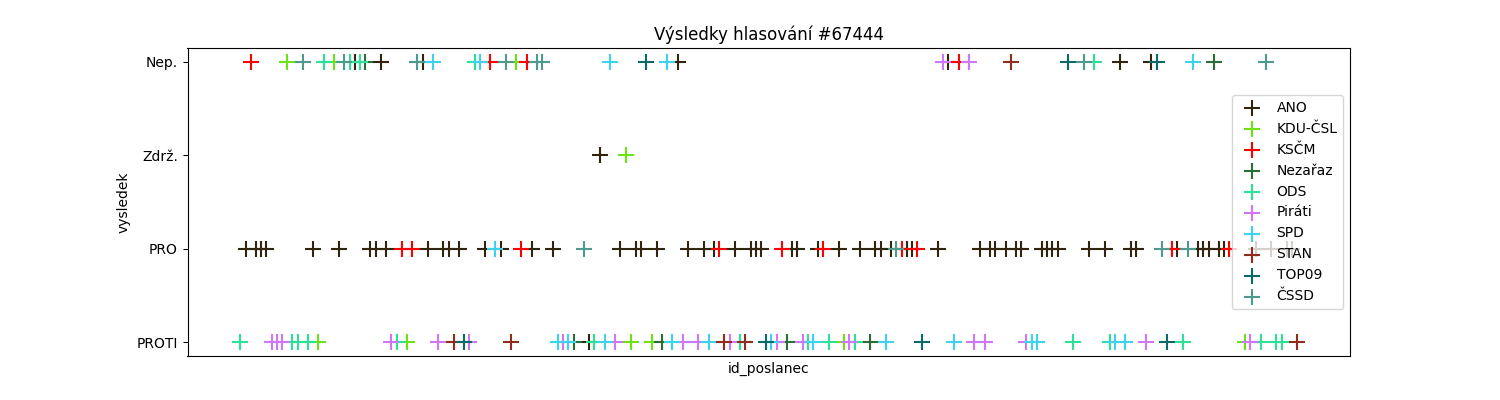
\includegraphics[width=1\textwidth]{obrazky-figures/analyza_hl_rozdilne.png}
    \caption{Vizualizace "přínosného"\ hlasování pro kalkulačku}
    \label{fig:analyza-rozdilne}
\end{figure}

\begin{figure}
    \centering
    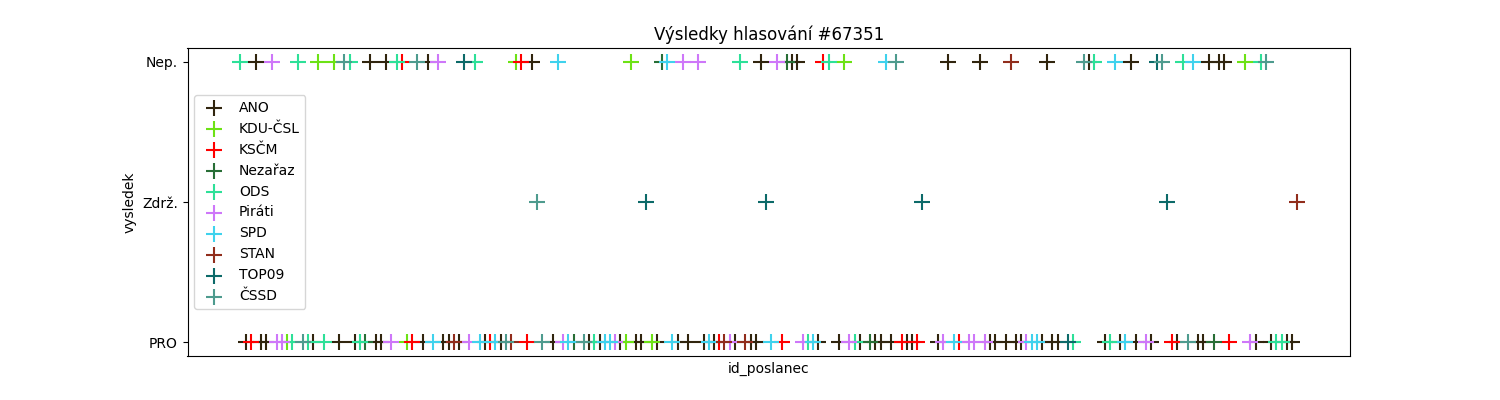
\includegraphics[width=1\textwidth]{obrazky-figures/analyza_hl_stejne.png}
    \caption{Vizualizace "nepodstatného"\ hlasování pro kalkulačku}
    \label{fig:analyza-stejne}
\end{figure}

\section{Způsob zpracování výsledků kalkulačky}
Uživatel bude "hlasovat"\ ve stejných hlasováních jako skuteční poslanci. Porovnání proto bude probíhat komparací výsledků kalkulačky s daty v databázi. Jelikož otázky se budou měnit velmi zřídka, bude k ukládání všech dat, potřebných pro výpočet výsledků, použita samostatná tabulka, působící jako určitý druh cache\footnote{cache: \url{https://cs.wikipedia.org/wiki/Cache}}, do které se vždy při aktualizaci otázek připraví všechno potřebné. Tímto způsobem se tak zredukují rozsáhlé SQL dotazy pro každého uživatele zvlášť na jednoduché čtení z jedné tabulky. 
\par Samotné zpracování bude probíhat tak, že po odeslání uživatelem k vyhodnocení bude do této tabulky vyslán SQL dotaz, žádající data o poslancích, kteří odpověděli alespoň na jednu z otázek shodně s uživatelem. Tito poslanci budou následně seřazeni podle počtu shodných odpovědí a tento počet převeden na procenta pro lepší orientaci. 
\par Pro strany bude postup podobný, rozdíl bude pouze v tom, že všechny jejich členy sečteme a zprůměrujeme.

\section{Způsob zpracování výsledků kalkulačky 2}
Uživatel bude "hlasovat"\ ve stejných hlasováních jako skuteční poslanci. Porovnávní proto bude probíhat komparací jeho voleb s hlasováním jednotlivých poslanců a stran u těch hlasování, kde uživatel uvedl svoji volbu. Tzn. pokud bude uživatel hlasovat například u \#67351 a \#67444, budou jeho výsledky porovnávny s výsledky poslanců pouze v těchto dvou konkrétních hlasováních. Následně se pro každého poslance vypočte procentuální shoda a výsledky se seřadí od té největší.

\par Pro porovnání se stranami bude nejprve potřeba pro každou najít nejčastější volbu reperzentující názor strany jako takové (či více v případě stejného počtu hlasů pro různé volby). Poté lze postupovat stejně jako u poslanců.




\section{Výběr vhodného serveru}
Aby aplikaci mohli používat lidé, musí být umístěna na veřejně přístupném serveru. Zde máme pro web obecně 3 možnosti:
\begin{itemize}
    \item Sdílený hosting\footnote{Hosting je zažitý název pro server na kterém je aplikace, či webová stránka umístěna}\\
    Jedná se o nejlevnější a obecně nejjednodušší možnou variantu. Daň za nízkou cenu je však ve sdílení hardwaru s dalšími aplikacemi. Z toho důvodu není možné dopředu předvídat dostupné prostředky a náročnější aplikace můžou skončit chybou kvůli jejich spotřebování ostatními. Také zde uživatel ve většině případů nemá kontrolu nad nainstalovanými aplikacemi a může využívat pouze omezený počet těch předpřipravených. Je zde také bezpečnostní riziko, protože data různých aplikací jsou na stejných úložištích. Jako příklad můžeme uvést například endora.cz\footnote{endora.cz: \url{https://www.endora.cz/}}
    \item Virtuální privátní server (VPS)\\
    U tohoto typu hostování je opět hardware serveru sdílen mezi několika aplikacemi. Každý uživatel však již má k dispozici vlastní virtualizovaný systém, který je oddělen od ostatních. Poskytuje tak uživateli mnohem více prostoru pro správu i lepší zabezpečení. Podstatně dražší, než sdílená verze. Např. cloudways.com\footnote{cloudwazys.com: \url{https://www.cloudways.com/en/}} 
    \item Dedikovaný sever\\
    Nejdražší varianta. Jde o kompletně vyčleněný hardware pro použití jedním zákazníkem. Zde má zákazník plnou kontrolu nad obsahem serveru a nainstalovanými aplikacemi. Například sh.cz\footnote{sh.cz: \url{https://www.sh.cz/dedikovane-servery}}
\end{itemize}

Jelikož framework Django nespadá do úplně běžných případů užití, většina sdílených řešení ho nepodporuje. Jako východisko se tedy nabízí buď využít školní server Eva, nebo sáhnout po nějakém dražším sdíleném.
\par Zejména z důvodu výhod naprosté kontroly nad systémem a jednoduchosti nasazení jsem zvolil digitalocean.com\footnote{digitalocean.com: \url{https://www.digitalocean.com/}}, kde se dostačující sdílený VPS server dá pořídit za 5\$ měsíčně.

\section{Doména}
Jelikož přístup na web přes IP adresu není moc praktický, potřebuje server zapamatovatelnou doménu, pod kterou ho lidé budou moci vyhledat. Domény s koncovkou .cz stojí obecně zhruba 200 korun ročně a koupit ji není nic složitého. 
\par Aby však web byl pod touto doménou dostupný, je třeba jí nejprve přidat záznam NS s odkazem na DNS servery\footnote{Dnes server je v podstatě překladač url adresy na IP adresu, viz \url{https://www.cloudflare.com/learning/dns/what-is-a-dns-server/}} zvoleného poskytovatele hostingu. Pro domény s koncovkou \texttt{.cz} je tato akce navíc specifická, protože nelze přidat jednotlivé DNS servery, nýbrž je potřeba vytvořit tzv. NSSET\footnote{Vytvoření NSSETu: \url{https://objednavka.forpsi.com/domain/cr-nsset.php}} a ten teprve přidat k záznamům pro doménu. Tím bude zajištěno, že každý dotaz hledající tuto URL adresu bude nasměrován správným směrem.

\par Aby DNS servery uměly hledanou URL adresu přeložit na IP adresu, je třeba na serveru nastavit záznamy typu A(IPV4), AAAA(IPV6) a NS. Toto nastavení lze například pro digitalocean.com vidět na obrázku \ref{fig:digitalocean-dns}.


\begin{figure}
    \centering
    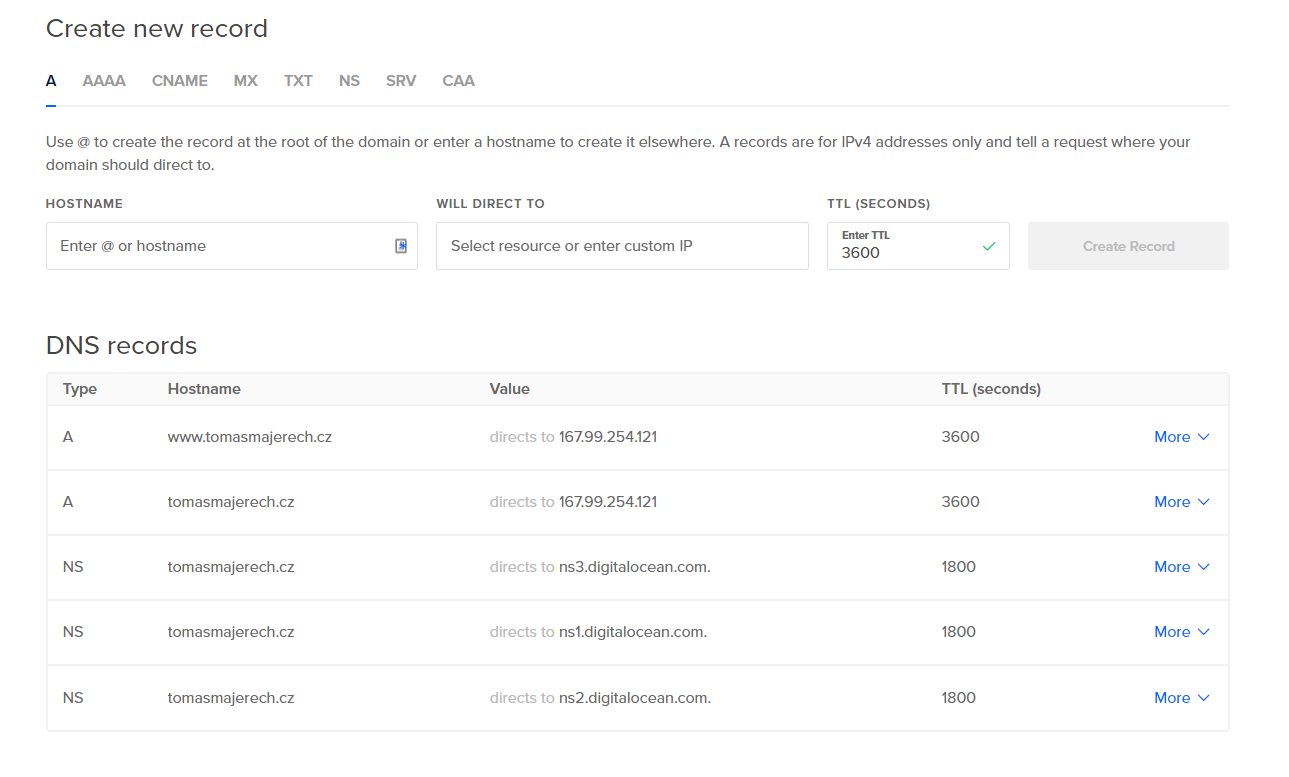
\includegraphics[width=0.9\textwidth]{obrazky-figures/digitaloceanDNSadmin.png}
    \caption{Rozhraní administrace DNS na webu digitalocean.com}
    \label{fig:digitalocean-dns}
\end{figure}

\section{Zprovoznění aplikace a domény na školním serveru}
\todo{Bude doplněno}

\section{?GDPR?}



\chapter{Nové myšlenky, které tato práce přináší (30 \%)}
\label{chap:novinky}



\chapter{Implementace a vyhodnocení (30 \%)}
\label{chap:implementace}




\section{Automatická aktualizace dat}
\todo{Dopsat script a popsat}


\chapter{Testování}
\label{chap:testovani}


\chapter{Závěr (1 strana)}
\label{chap:zaver}